\documentclass[9 pt,makeindex]{beamer}
\usepackage{makeidx}
\makeindex

\usepackage{latexcolors}

% 背景图片
\usepackage{tikz}
\pgfdeclareimage[height=\paperheight,width=\paperwidth]{myimage}{figures/Kohrvirab.jpg}
\usebackgroundtemplate{\tikz\node[opacity=0.1] {\pgfuseimage{myimage}};}

\usepackage{multicol}   %目录分栏

\usepackage[space, hyperref, UTF8]{ctex}	%中文支持

% 数理
\usepackage{amsmath,amssymb,amsthm}
\usepackage{esint}		% \oiint
\usepackage{amsfonts}
\usepackage{latexsym}
\usepackage{extarrows}  	%长等号上写字\xlongequal{文字}
\usepackage{physics}
\usepackage{upgreek}    	%直立的希腊字母\upalpha
\usepackage{bm}     		%加粗\bm{}
\usepackage{slashed}    	%Dirac slash

%插入 Mathematica 代码请先在当前目录下放入 mmacells.sty
%\usepackage{mmacells}
%\usepackage[framed,numbered,autolinebreaks,useliterate]{mcode}  %MATLAB 官方宏包
% \usepackage{listings}		% 插入代码:已过时

\usepackage{graphicx}   %插入图片的宏包
\usepackage{float}      %设置图片浮动位置的宏包
\usepackage{subfigure}  %插入多图时用子图显示的宏包

%\usepackage[xllnames]{xcolor}

%\usepackage[hidelinks]{hyperref}

%插入 emoji 表情:使用 \LuaLaTeX,\Memoji{🎄}
%\usepackage{metalogo}
%\usepackage{fontspec}
%\setmainfont{Comic Sans MS}
%\newfontfamily\emojifont{Segoe UI Emoji}[Renderer=Harfbuzz]
%\newcommand{\emoji}[1]{\emojifont #1}
%\newcommand{\Memoji}[1]{\ifmmode \text{\emoji{#1}} \else \emoji{#1}\fi}

\usetheme{Goettingen}
\usecolortheme{crane}

\title[文献调研]{2022寒假文献调研}
\subtitle{光电器件中的波长选择}
\author{冯哲}
\date{\today}
\institute{河海大学 理学院}
%\titlegraphic{\includegraphics[width=0.17\textwidth]{ias.pdf}}

% \usepackage{syntonly}
% \syntaxonly %声明后,仅检查语法是否正确

\includeonly{texes/sesankongzhenliechonggou.tex, texes/End.tex} % 仅真正编译这几个文件

\begin{document}

\frame{\titlepage}

\begin{frame}
    \frametitle{Outline}
    \tableofcontents
\end{frame}
%\section{逐篇介绍}
%\sectionpage

\section{窄带滤光片}

\subsection{基于可调谐滤光片的显微光谱仪}
\subsubsection{声光可调谐(AOTFs)}
\begin{frame}[c]
    \frametitle{小型固态近红外光谱仪的设计:概要}
    \begin{itemize}
        \item Zhang, H.;  Wang, X.;  Soos, J.; Crisp, J., Design of a \textcolor{purple}{miniature} solid state \textcolor{red}{NIR} spectrometer. SPIE: 1995; Vol. 2475.
        \item \textcolor{blue}{重要性:}灵敏度高、速度快、无需移动部件、无需机械调整的自校准。
        \item \textcolor{blue}{意义:}可以应用于航空航天领域。
    \end{itemize}
    \begin{figure}[H] %H为当前位置,!htb为忽略美学标准,htbp为浮动图形
        \centering %图片居中
        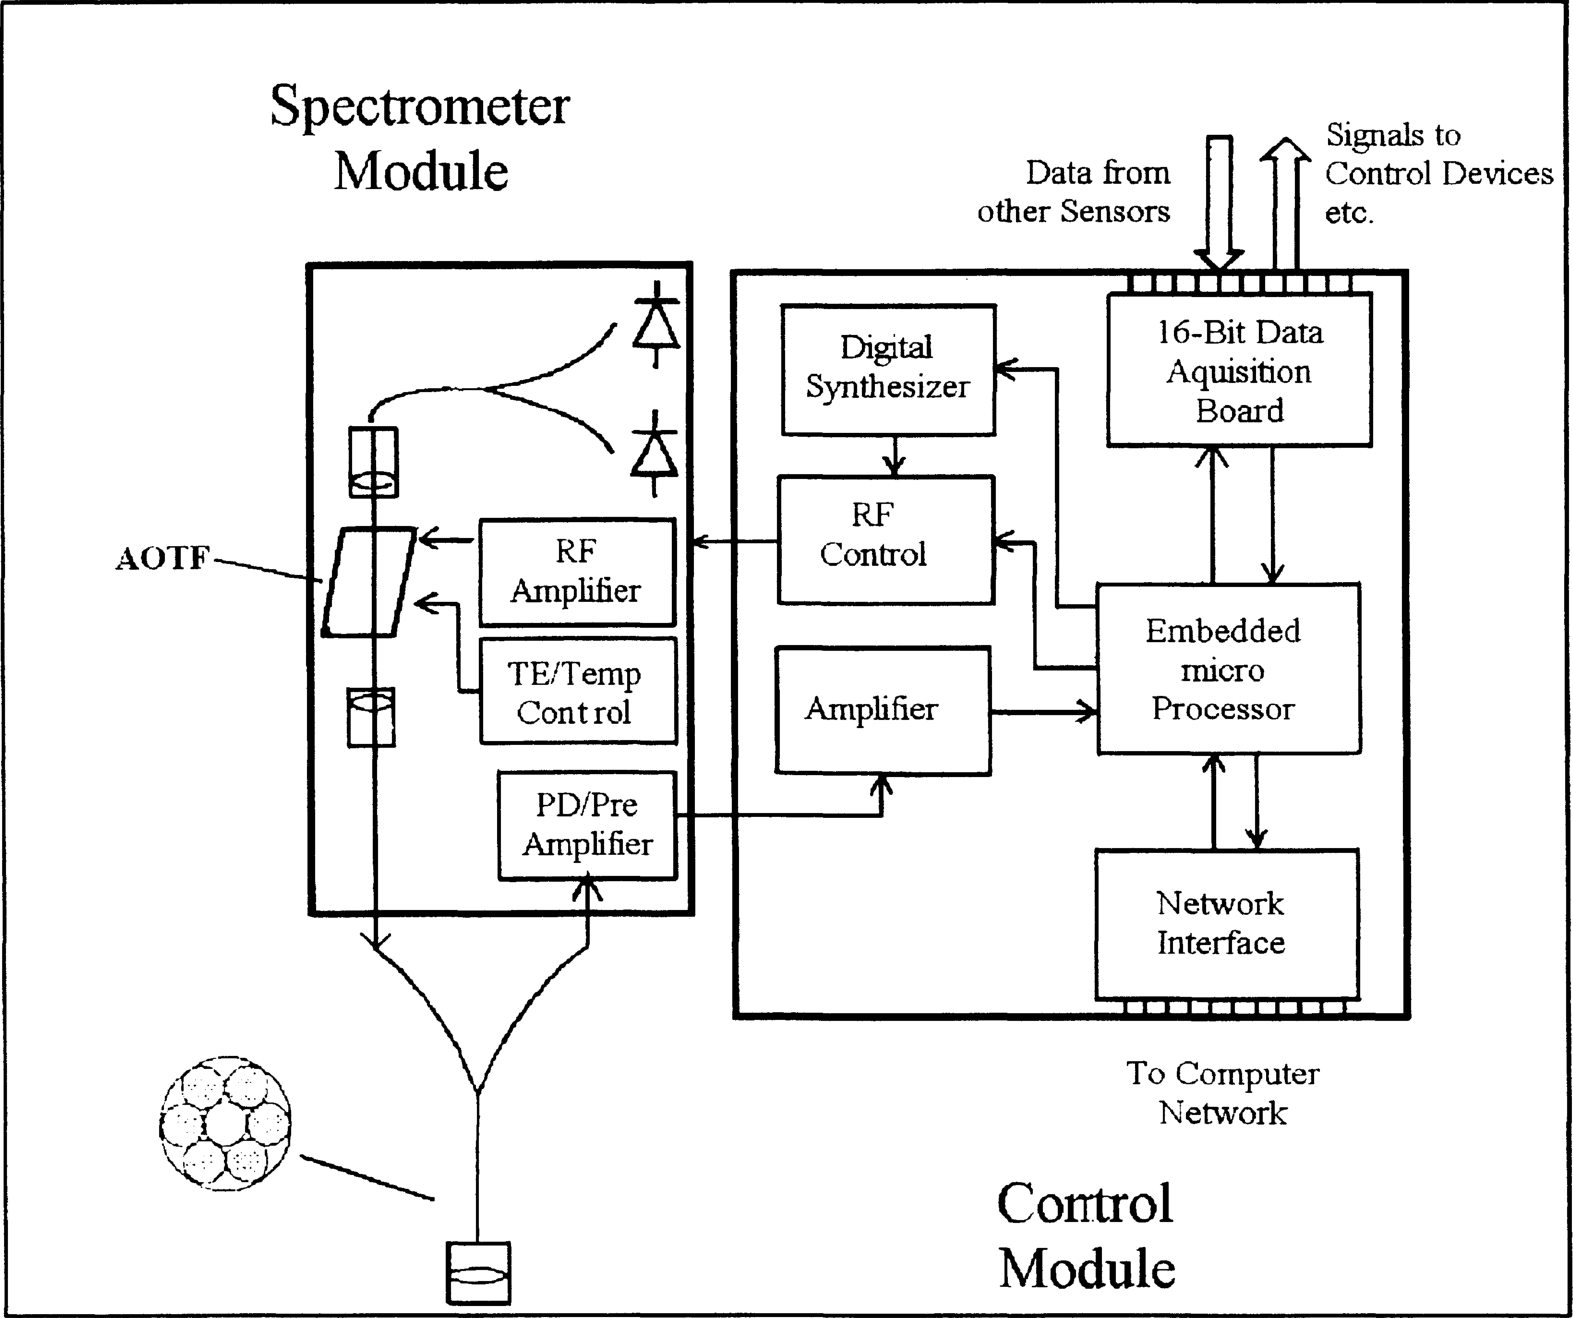
\includegraphics[width=.8\textwidth]{figures/Design of a miniature solid state NIR spectrometer_1.png} %插入图片,[]中设置图片大小,{}中是图片文件名
    \end{figure}
\end{frame}

\begin{frame}[c]
    \frametitle{小型固态近红外光谱仪的设计:原理}
    \begin{enumerate}
        \item 特定频率的信号激励
        \item $\mathrm{TeO}_2$ 晶体中产生声波
        \item 形成周期性的折射率,相当于光子晶体或光栅
        \item 波长满足相位条件的光通过
    \end{enumerate}
    \begin{figure}[H] %H为当前位置,!htb为忽略美学标准,htbp为浮动图形
        \centering %图片居中
        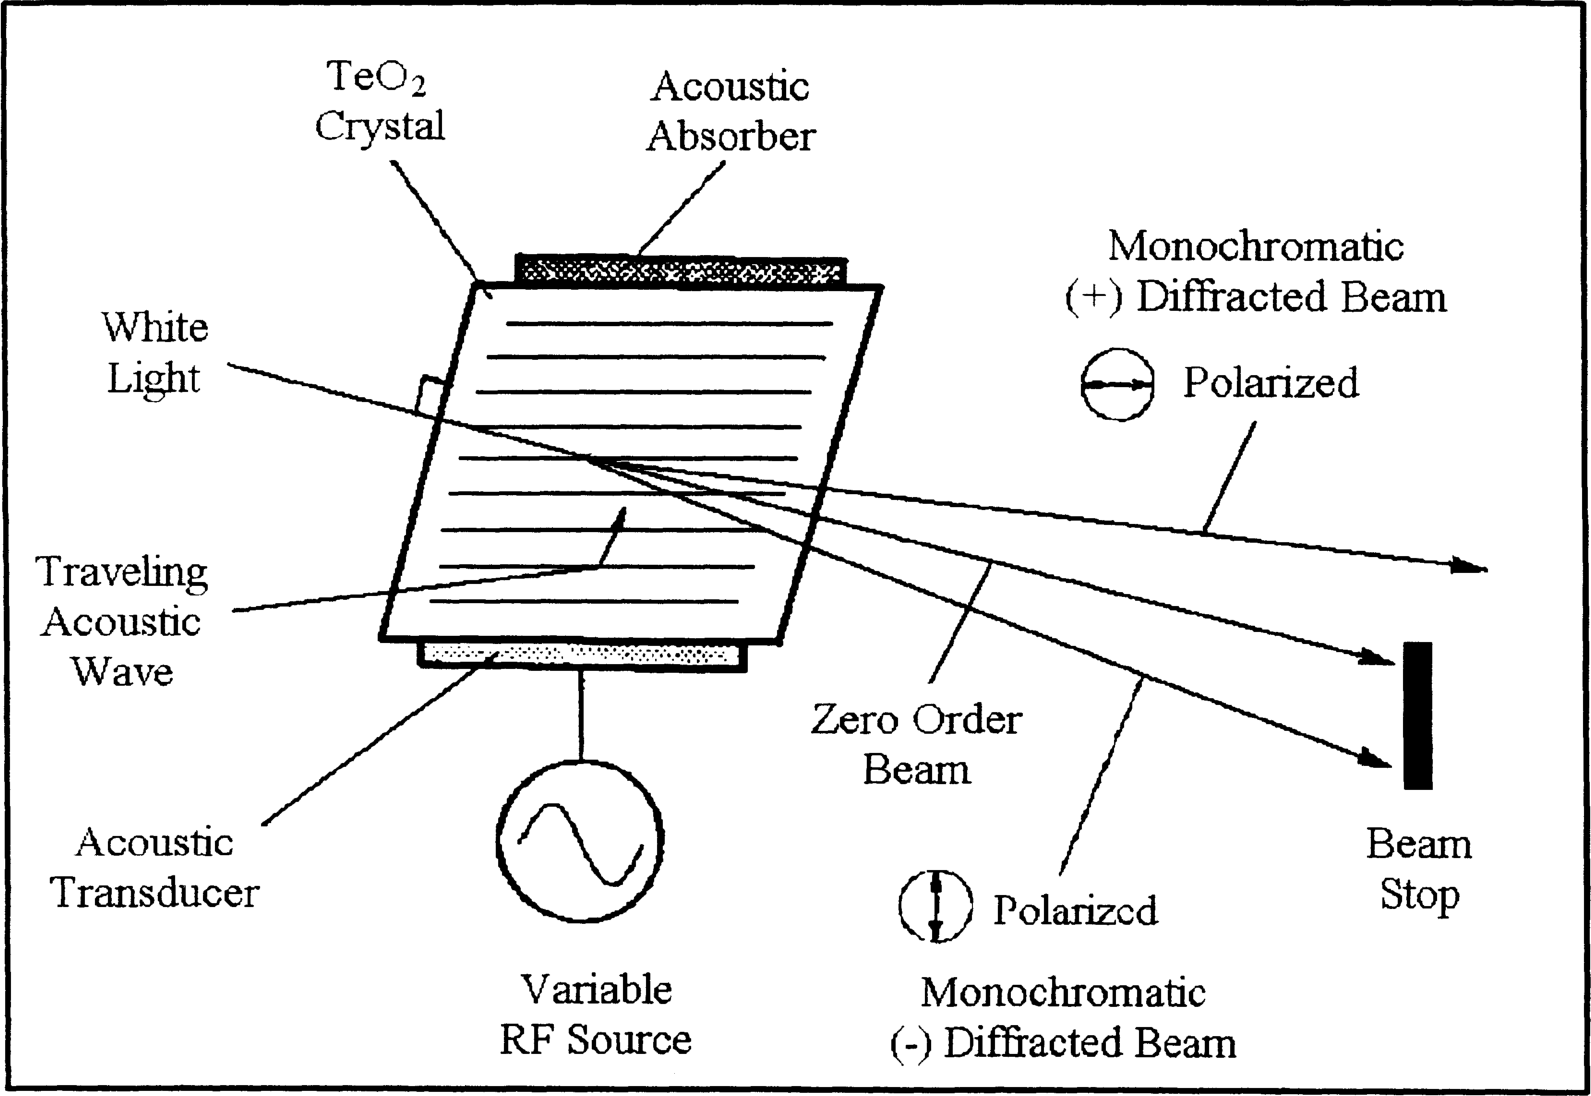
\includegraphics[width=.8\textwidth]{figures/Design of a miniature solid state NIR spectrometer_3.png} %插入图片,[]中设置图片大小,{}中是图片文件名
    \end{figure}
\end{frame}

\begin{frame}[c]
    \frametitle{小型固态近红外光谱仪的设计:实验细节}
    \begin{columns}
        \begin{column}{.4\textwidth}
            LED 代替卤钨灯作光源:
            \begin{itemize}
                \item 节能
                \item 亮度高
                \item 寿命长
                \item 带宽窄
                \item 发光面积小
                \item 稳定
            \end{itemize}
        \end{column}
        \begin{column}{.6\textwidth}
            \begin{figure}[H] %H为当前位置,!htb为忽略美学标准,htbp为浮动图形
                \centering %图片居中
                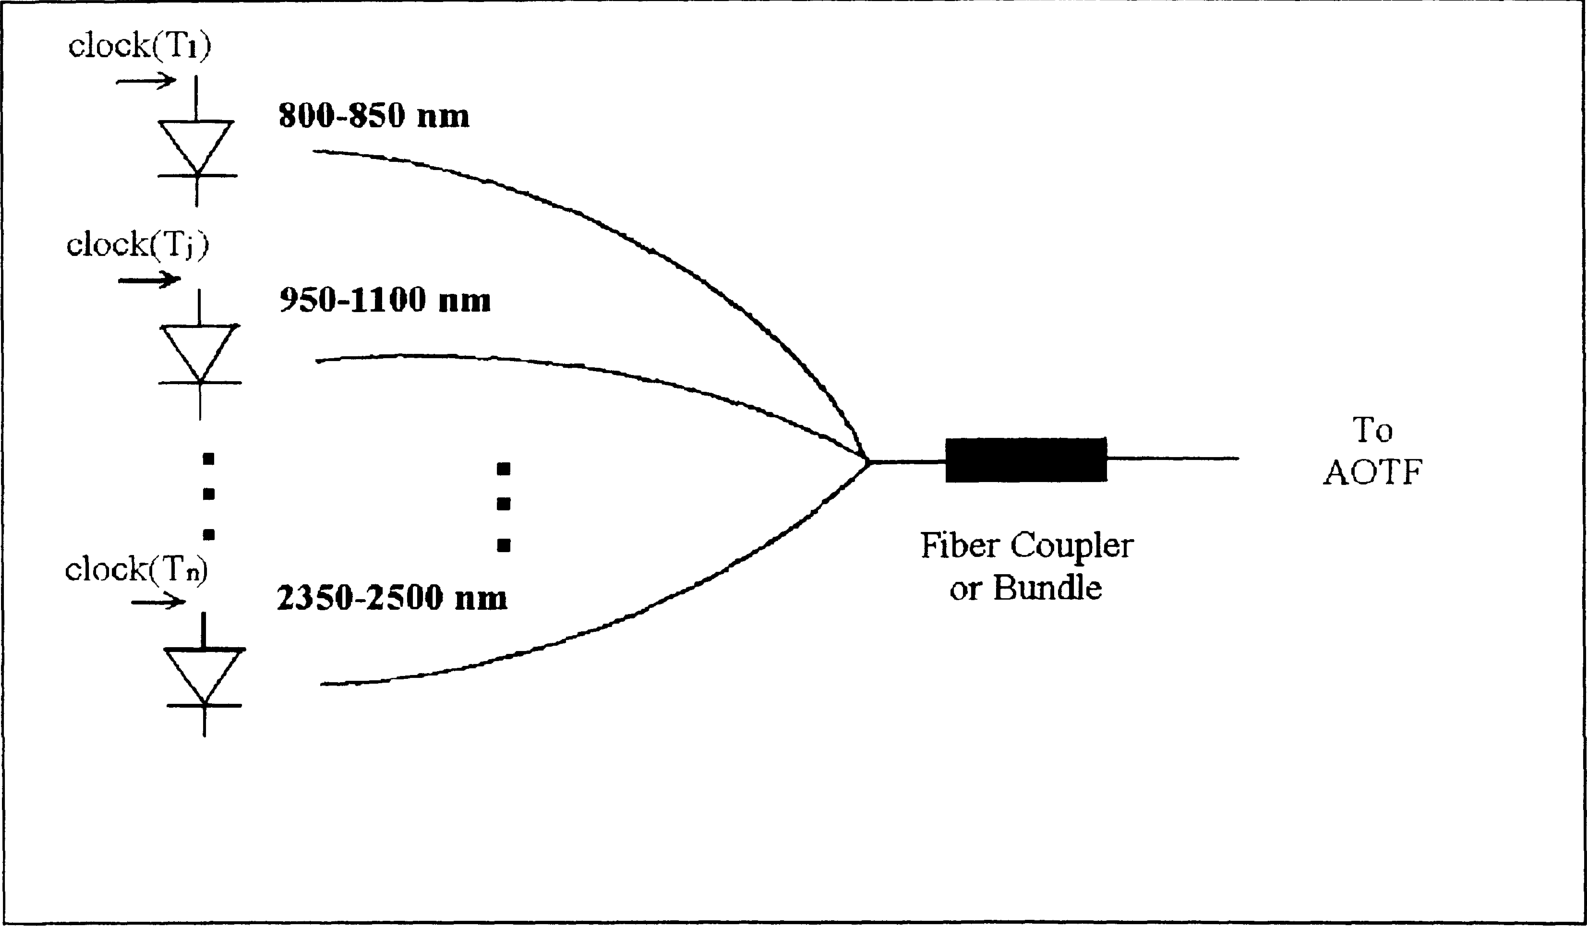
\includegraphics[width=1.\textwidth]{figures/Design of a miniature solid state NIR spectrometer_2.png} %插入图片,[]中设置图片大小,{}中是图片文件名
            \end{figure}
        \end{column}
    \end{columns}
\end{frame}
\subsubsection{液晶可调谐(LCTFs)}
\subsubsection{$\mathrm{LiNbO}_3$ 可调谐双腔 FP}
\begin{frame}[c]
    \frametitle{多腔红外电光可调谐滤波器:概要}
    \begin{columns}
        \begin{column}{.6\textwidth}
            \begin{itemize}
                \item Gunning, W.; Yeh, P., \textcolor{red}{Multiple-Cavity} \textcolor{pink}{Infrared} \textcolor{purple}{Electro-Optic Tunable} Filter. SPIE: 1980; Vol. 0202.
                \item \textcolor{blue}{重要性:}规避了使用机械调谐结构带来的对温度和颤噪声的敏感。
                \item \textcolor{blue}{瓶颈:}工作波段太窄()。只有不到 $20\ \mathrm{nm}$
                \item \textcolor{blue}{意义:}具有潜在的高传输能力。
                \item \footnotesize{使用的材料:铌酸锂 $\mathrm{LiNbO}_3$,其单晶为光波导,是重要的非线性光学应用材料}
            \end{itemize}
        \end{column}
        \begin{column}{.4\textwidth}
            \begin{figure}[H] %H为当前位置,!htb为忽略美学标准,htbp为浮动图形
                \centering %图片居中
                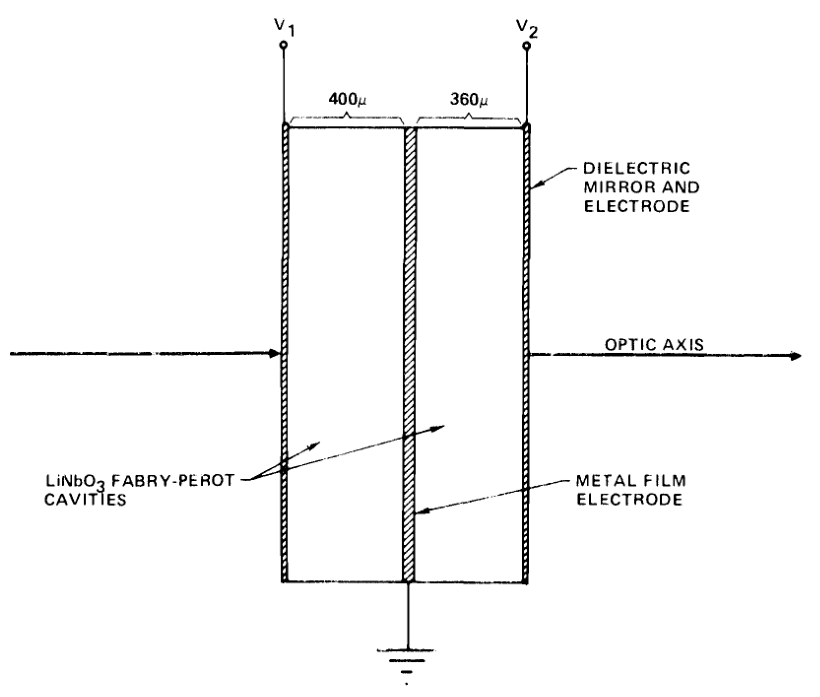
\includegraphics[width=1.\textwidth]{figures/Multiple-Cavity Infrared Electro-Optic Tunable Filter_2.png} %插入图片,[]中设置图片大小,{}中是图片文件名
                \caption{器件结构}
            \end{figure}
        \end{column}
    \end{columns}

    \begin{itemize}
        \item 原理:铌酸锂 $\mathrm{LiNbO}_3$ 是一种特殊的光学材料,在外电场的激励下可产生折射率的改变,由此改变整个谐振腔的共振波长
    \end{itemize}
    器件结构(介质腔相当厚):light $\downarrow$
    \begin{itemize}
        \item Ni 电极 $\rightarrow$ 介质反射镜
        \item $400\ \mathrm{\mu m}\ \mathrm{LiNbO}_3$
        \item $15\ \mathrm{nm}\ \mathrm{Ag}$
        \item $360\ \mathrm{\mu m}\ \mathrm{LiNbO}_3$
        \item 介质反射镜 $\rightarrow$ Ni 电极
    \end{itemize}
\end{frame}

\begin{frame}[c]
    \frametitle{多腔红外电光可调谐滤波器:过程细节}
    \textrm{Ni} 和 \textrm{Ag} 薄膜效果的比较:
    \begin{itemize}
        \item 使用较高 $k/n$ 的值的金属材料效果较好($\mathrm{Ag: }20,\ \mathrm{Ni: }2.3$)
    \end{itemize}

    \begin{figure}[H] %H为当前位置,!htb为忽略美学标准,htbp为浮动图形
        \centering %图片居中
        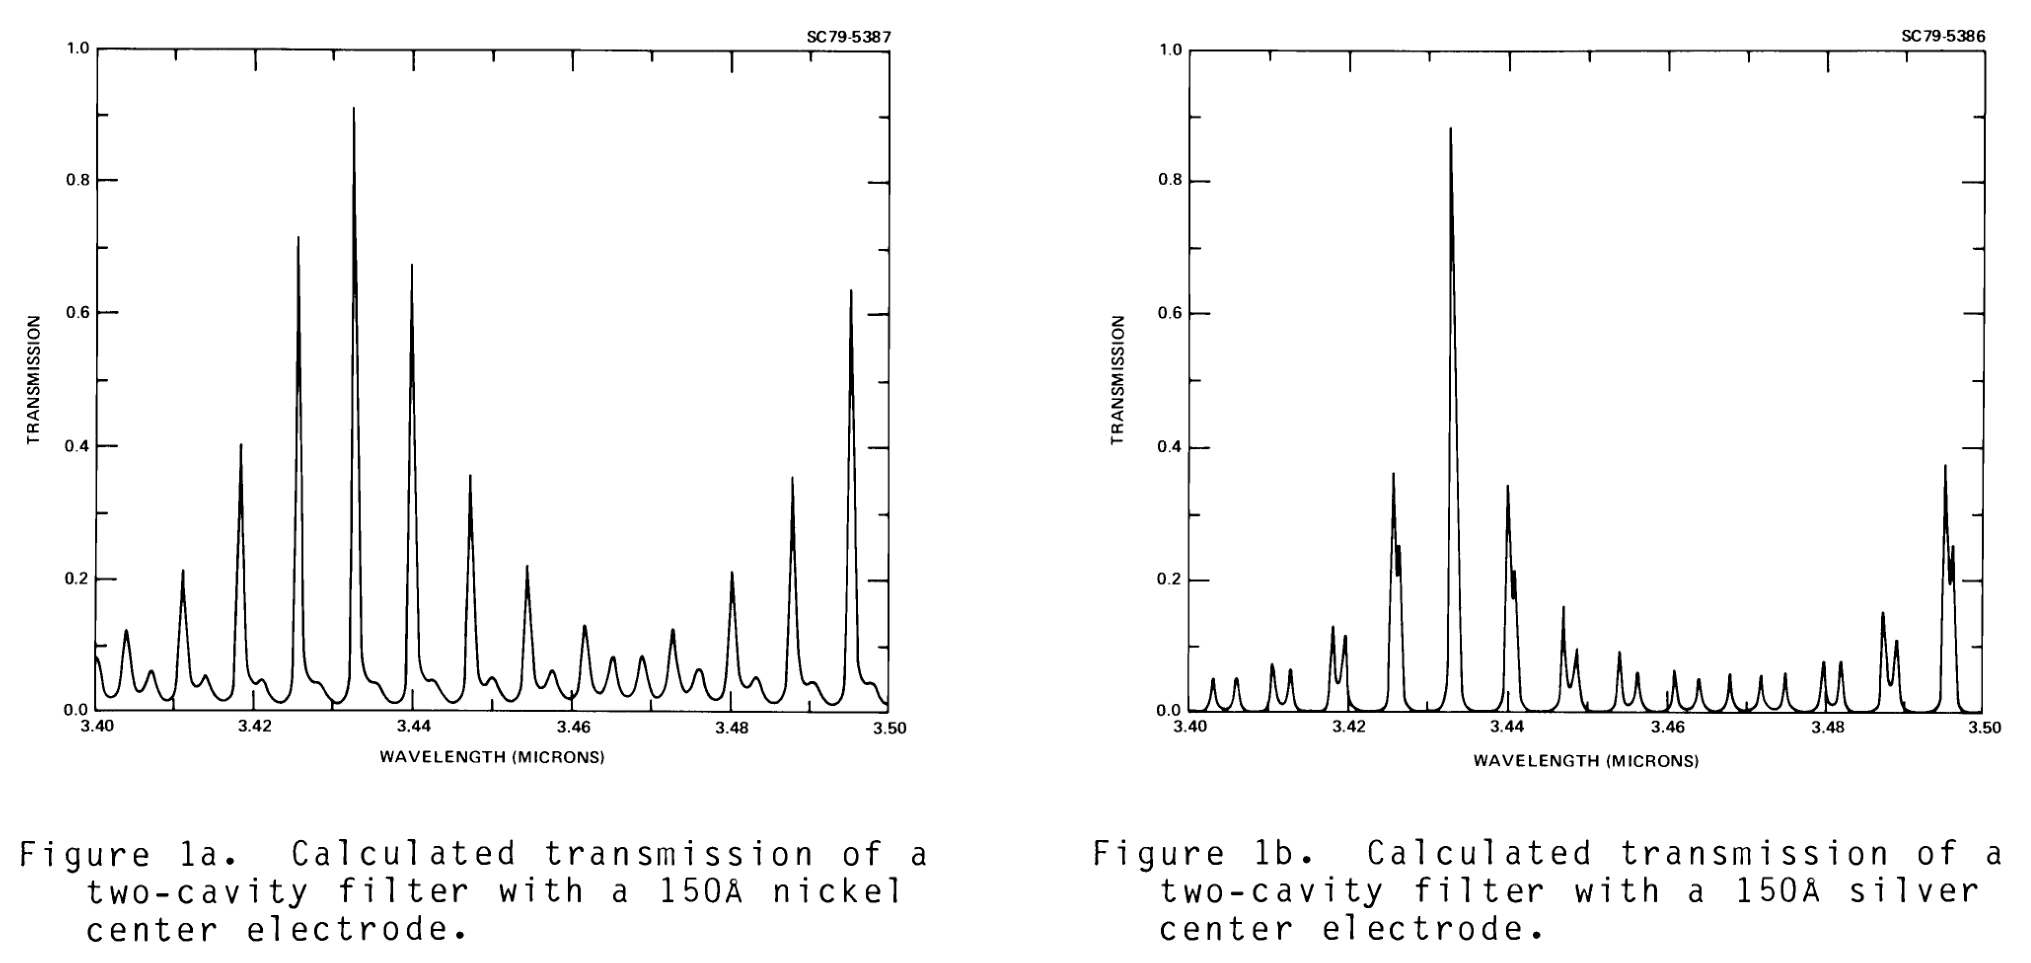
\includegraphics[width=1.\textwidth]{figures/Multiple-Cavity Infrared Electro-Optic Tunable Filter_1.png} %插入图片,[]中设置图片大小,{}中是图片文件名
        \caption{\textrm{Ni} 和 \textrm{Ag} 薄膜的比较}
    \end{figure}
\end{frame}

\begin{frame}[c]
    \frametitle{多腔红外电光可调谐滤波器:仪器性能}
    \begin{itemize}
        \item 可以看到,仪器工作波段只有不到 $20\ \mathrm{nm}$,有待发展。
    \end{itemize}

    \begin{figure}[H] %H为当前位置,!htb为忽略美学标准,htbp为浮动图形
        \centering %图片居中
        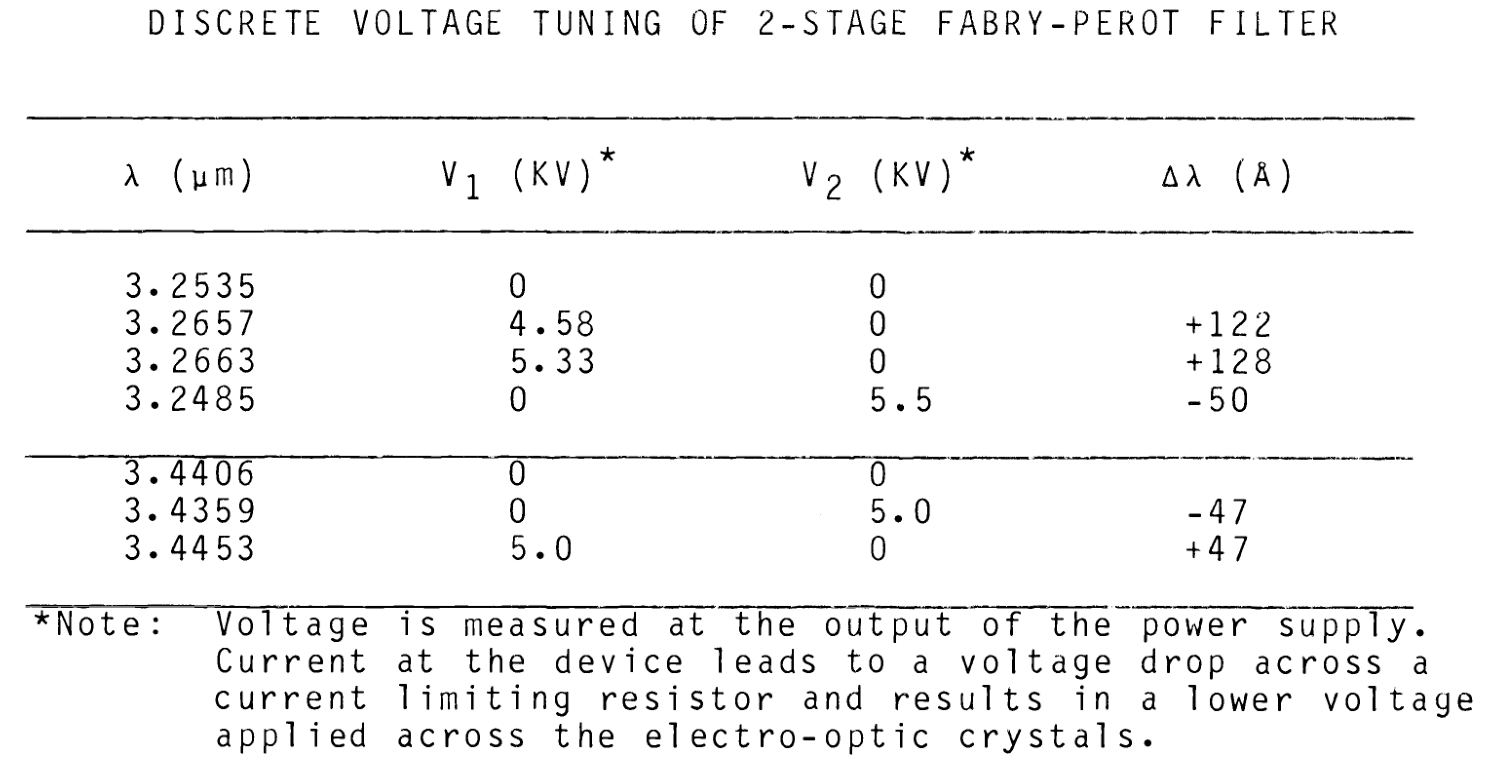
\includegraphics[width=1.\textwidth]{figures/Multiple-Cavity Infrared Electro-Optic Tunable Filter_3.png} %插入图片,[]中设置图片大小,{}中是图片文件名
        \caption{仪器性能}
    \end{figure}
\end{frame}
\subsubsection{$\mathrm{LiNbO}_3$ 可编程可调谐}
\begin{frame}[c]
    \frametitle{基于铌酸锂的可编程多波长可调谐滤波器设计:概述}
    \begin{columns}
        \begin{column}{.6\textwidth}
            \begin{itemize}
                \item Yao, Y.;  Hou, J.;  Liu, H.;  Zhang, A.;  Liu, B.;  Zhang, H.; Liu, J., Design of \textcolor{purple}{programmable} multi-wavelength tunable filter on \textcolor{red}{lithium niobate}. Results in Physics 2019, 15, 102741.
                \item \textcolor{blue}{创新点:}通过对电极对进行编码,实现了谐振波长数和波长间距的可编程化。
                \item \textcolor{blue}{瓶颈:}工作波段过窄(文章中展示的只有几个 $\mathrm{nm}$)。
                \item \textcolor{blue}{意义:}可以应用于开发具有快速调谐速度的基于铌酸锂的单芯片。
            \end{itemize}
        \end{column}
        \begin{column}{.4\textwidth}
            \begin{figure}[H] %H为当前位置,!htb为忽略美学标准,htbp为浮动图形
                \centering %图片居中
                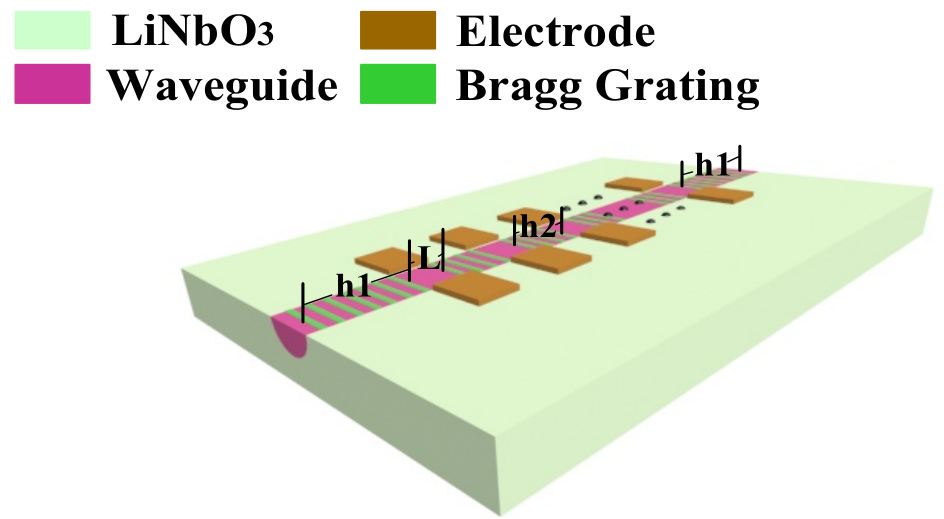
\includegraphics[width=1.\textwidth]{figures/Design of programmable multi-wavelength tunable filter on lithium niobate_1.png} %插入图片,[]中设置图片大小,{}中是图片文件名
                \caption{器件示意图}
            \end{figure}
        \end{column}
    \end{columns}

    \begin{itemize}
        \item 原理:光通过每个宽为 $L$ 的波导会产生相移\[\varphi=\frac{4\pi}{\lambda}(n_{\mathrm{eff}}-\frac{\gamma_{33}n_{\mathrm{eff}}^3V\Gamma}{2d})L\]通过改变 $V$ 来调整目标波长
    \end{itemize}
\end{frame}

\begin{frame}[c]
    \frametitle{基于铌酸锂的可编程多波长可调谐滤波器设计:滤波性能}

    波长选择性较好,透射峰极尖锐,但是工作波长太窄:

    \begin{columns}
        \begin{column}{0.5\textwidth}
            \begin{figure}[H] %H为当前位置,!htb为忽略美学标准,htbp为浮动图形
                \centering %图片居中
                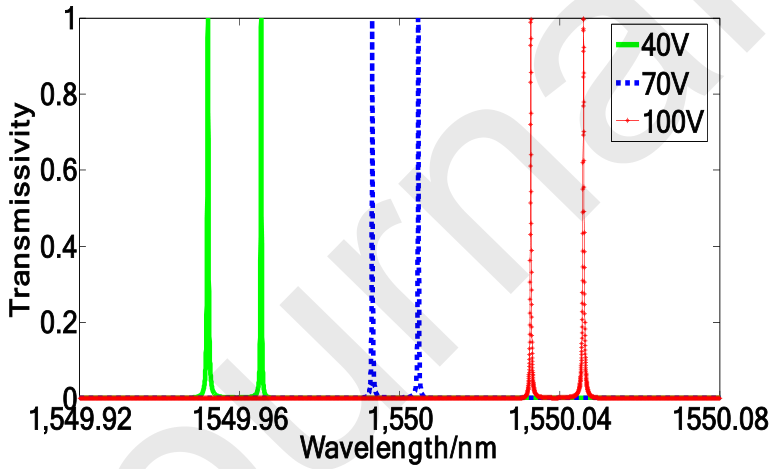
\includegraphics[width=.9\textwidth]{figures/Design of programmable multi-wavelength tunable filter on lithium niobate_2.png} %插入图片,[]中设置图片大小,{}中是图片文件名
            \end{figure}
            \begin{figure}[H] %H为当前位置,!htb为忽略美学标准,htbp为浮动图形
                \centering %图片居中
                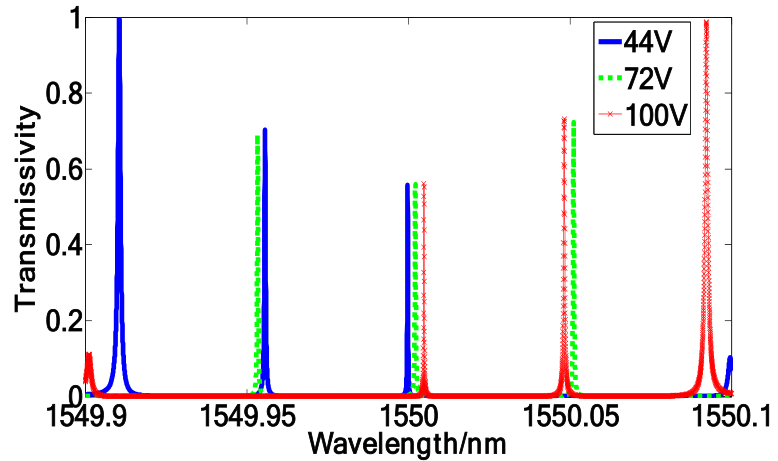
\includegraphics[width=.9\textwidth]{figures/Design of programmable multi-wavelength tunable filter on lithium niobate_3.png} %插入图片,[]中设置图片大小,{}中是图片文件名
                \caption{改变电压 $V$ 的效果}
            \end{figure}
        \end{column}
        \begin{column}{0.5\textwidth}
            \begin{figure}[H] %H为当前位置,!htb为忽略美学标准,htbp为浮动图形
                \centering %图片居中
                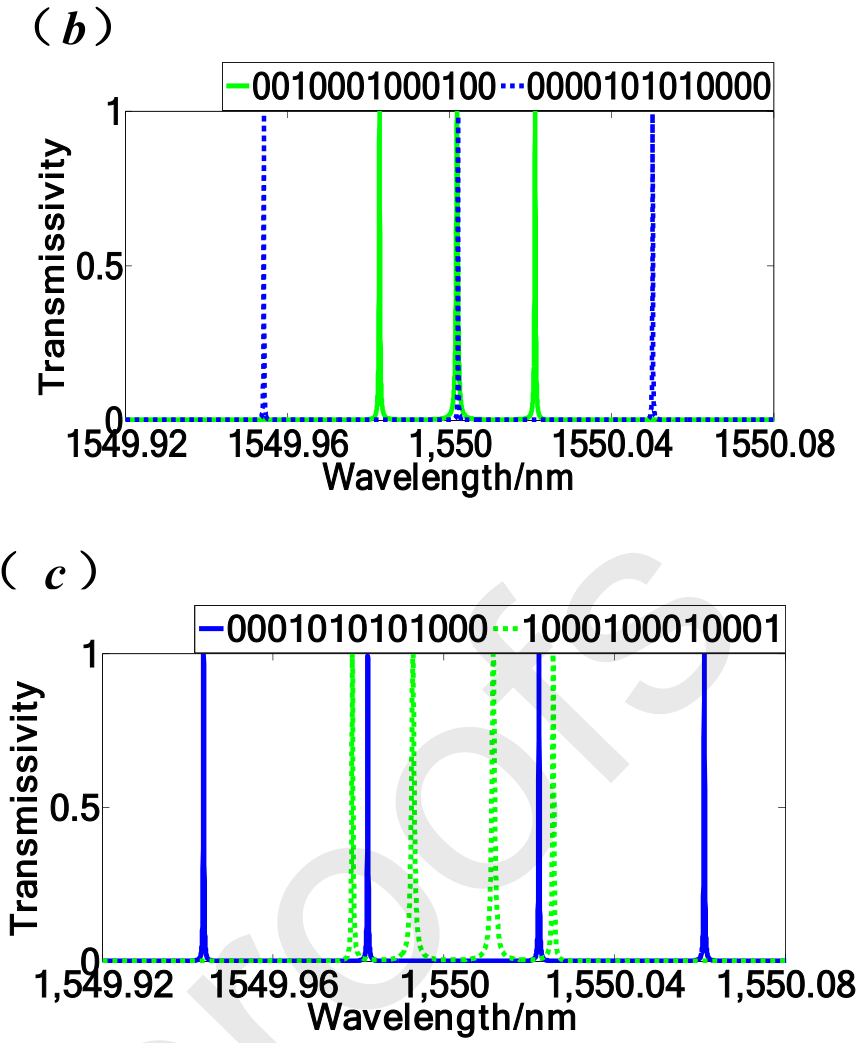
\includegraphics[width=.9\textwidth]{figures/Design of programmable multi-wavelength tunable filter on lithium niobate_4.png} %插入图片,[]中设置图片大小,{}中是图片文件名
                \caption{上面的编码指的是“第几个波导加电压”}
            \end{figure}
        \end{column}
    \end{columns}

\end{frame}
\subsubsection{有机液晶可调谐}
\begin{frame}[c]
    \frametitle{液晶可调谐光谱滤波器:可见光和红外操作}
    \begin{columns}
        \begin{column}{.6\textwidth}
            \begin{itemize}
                \item Gunning, W.;  Pasko, J.; Tracy, J., A \textcolor{purple}{Liquid Crystal} \textcolor{red}{Tunable} Spectral Filter: \textcolor{pink}{Visible And Infrared} Operation. SPIE: 1981; Vol. 0268.
                \item \textcolor{blue}{重要性:}较小范围内的电压调节即可实现较大范围的工作波长。
                \item \textcolor{blue}{瓶颈:}液晶的光学参数与温度有很强的相关性,因此需要研究与热效应有关的问题。
                \item \textcolor{blue}{创新点:}之前的器件在调节通带光谱时所需要的电压非常大,液晶的使用克服了这一限制。
                \item \textcolor{blue}{意义:}有望设计出新的设备,尤其是多个谐振腔的滤波器。
                \item \footnotesize{所使用的材料:\textrm{4-Cyano,-4'-$\eta$-pentylbiphenyl}(4-羟基,-4'-$\eta$-戊基联苯)}
            \end{itemize}
        \end{column}
        \begin{column}{.4\textwidth}
            \begin{figure}[!htb] %H为当前位置,!htb为忽略美学标准,htbp为浮动图形
                \centering %图片居中
                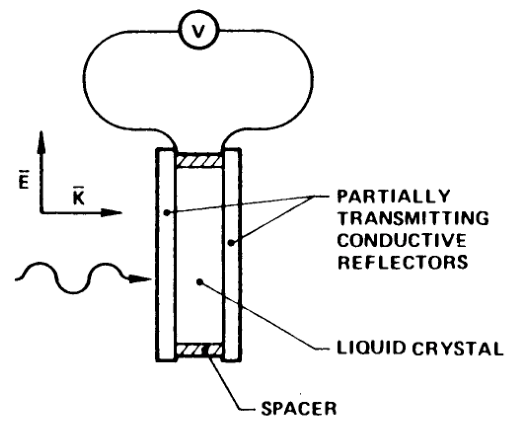
\includegraphics[width=1.\textwidth]{figures/A Liquid Crystal Tunable Spectral Filter Visible And Infrared Operation_1.png} %插入图片,[]中设置图片大小,{}中是图片文件名
                \caption{仪器结构示意图} %最终文档中希望显示的图片标题
            \end{figure}
        \end{column}
    \end{columns}
\end{frame}

\begin{frame}[c]
    \frametitle{液晶可调谐光谱滤波器:可见光和红外操作}
    此仪器是上一篇文章仪器的改进,变化在于谐振腔所使用的介质材料不同。
    \begin{itemize}
        \item 施加不同大小的电压,液晶分子(极化)取向的变化不同。
        \item 有效折射率:$\frac{1}{n(\theta)^2}=\frac{1}{n_\mathrm{o}^2}\cos^2\theta+\frac{1}{n_\mathrm{e}^2}\sin^2\theta$
        \item 典型值:$n_{\mathrm{e}}-n_{\mathrm{o}}=0.2$
    \end{itemize}

    \begin{columns}
        \begin{column}{.5\textwidth}
            \begin{figure}[!htb] %H为当前位置,!htb为忽略美学标准,htbp为浮动图形
                \centering %图片居中
                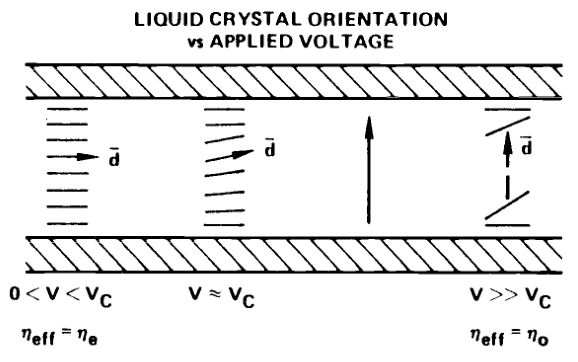
\includegraphics[width=1.\textwidth]{figures/A Liquid Crystal Tunable Spectral Filter Visible And Infrared Operation_2.png} %插入图片,[]中设置图片大小,{}中是图片文件名
                \caption{原理示意图} %最终文档中希望显示的图片标题
            \end{figure}
        \end{column}
        \begin{column}{.5\textwidth}
            \begin{figure}[!htb] %H为当前位置,!htb为忽略美学标准,htbp为浮动图形
                \centering %图片居中
                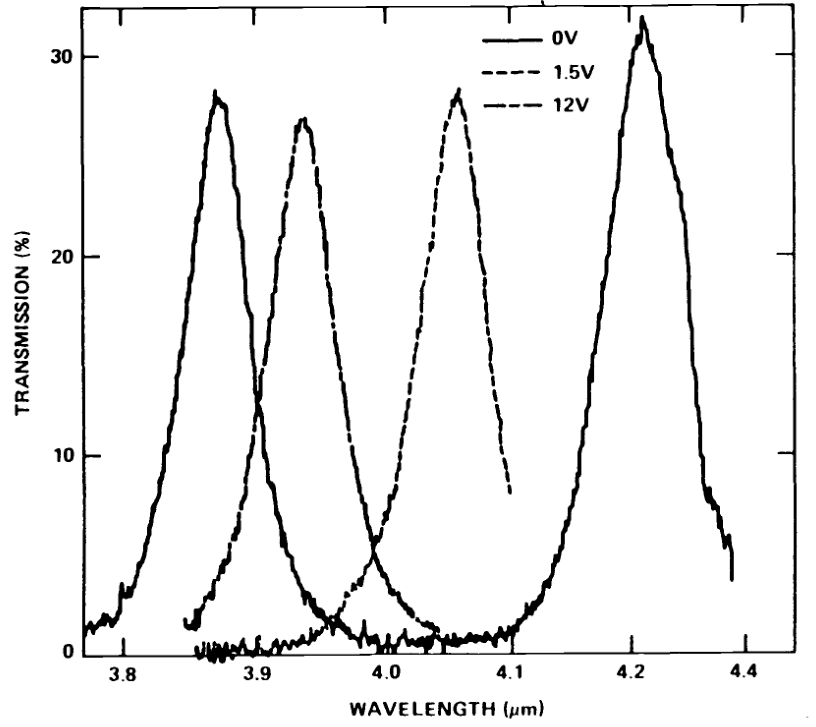
\includegraphics[width=1.\textwidth]{figures/A Liquid Crystal Tunable Spectral Filter Visible And Infrared Operation_3.png} %插入图片,[]中设置图片大小,{}中是图片文件名
                \caption{测试结果} %最终文档中希望显示的图片标题
            \end{figure}
        \end{column}
    \end{columns}
    \begin{itemize}
        \item可以看到,对于上一篇文章来说,现在的仪器用小得多的电压变化实现了大得多的通带波长调节。
    \end{itemize}
\end{frame}
\subsubsection{多孔硅角度可调谐}
\begin{frame}[c]
    \frametitle{基于多孔硅可调谐光学滤光片的微光谱仪:概述}
    \begin{columns}
        \begin{column}{.6\textwidth}
            \begin{itemize}
                \item Lammel, G.;  Schweizer, S.; Renaud, P., Microspectrometer based on a \textcolor{purple}{tunable optical filter} of \textcolor{red}{porous silicon}. Sensors and Actuators A: Physical 2001, 92 (1), 52-59.
                \item \textcolor{blue}{重要性:}降低了工艺复杂度和成本。
                \item \textcolor{blue}{创新点:}\begin{itemize}
                          \item 通过改变滤波片的角度调节通带波长。
                          \item 采用多孔硅批处理技术,只需两个光刻步骤即可制作出可调谐滤光片。
                          \item 只需要使用一个探测器,降低了成本。
                      \end{itemize}
                \item \textcolor{blue}{意义:}消除了常见的增益变化和补偿问题。
            \end{itemize}
        \end{column}
        \begin{column}{.4\textwidth}
            \begin{figure}[!htb] %H为当前位置,!htb为忽略美学标准,htbp为浮动图形
                \centering %图片居中
                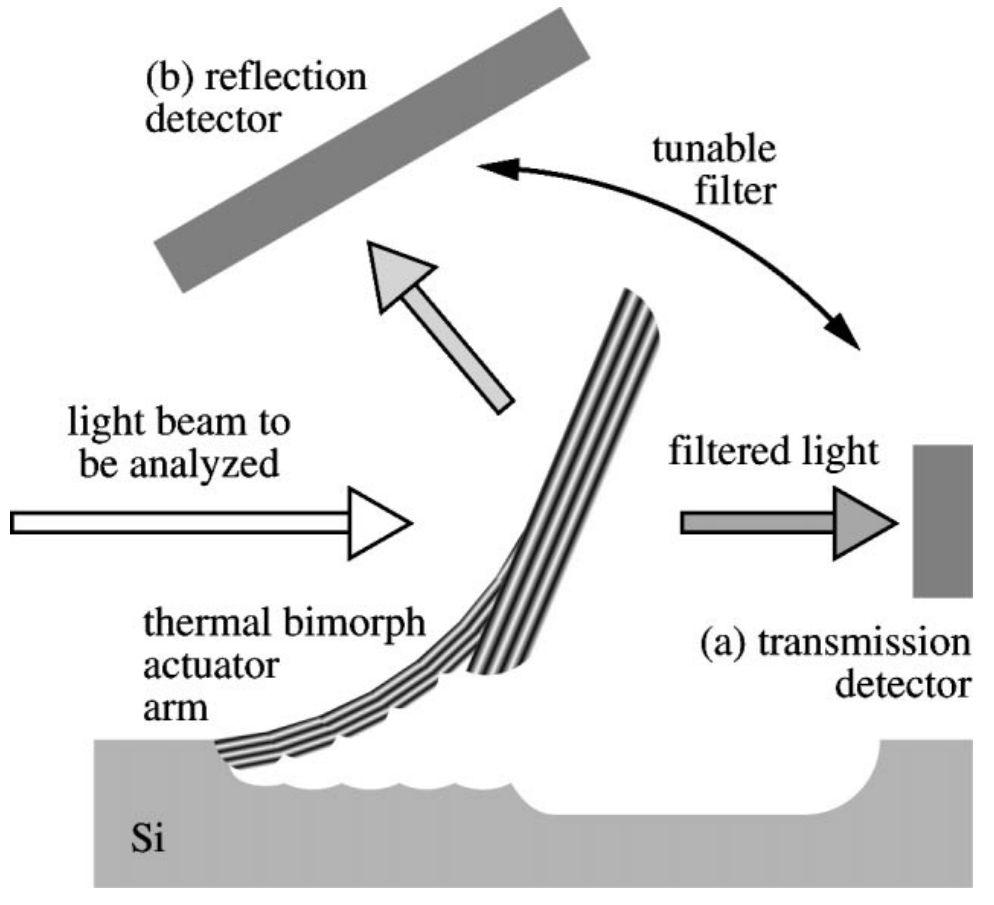
\includegraphics[width=1.\textwidth]{figures/Microspectrometer based on a tunable optical filter of porous silicon_1.png} %插入图片,[]中设置图片大小,{}中是图片文件名
                \caption{仪器结构示意图} %最终文档中希望显示的图片标题
            \end{figure}
        \end{column}
    \end{columns}

    \begin{figure}[!htb] %H为当前位置,!htb为忽略美学标准,htbp为浮动图形
        \centering %图片居中
        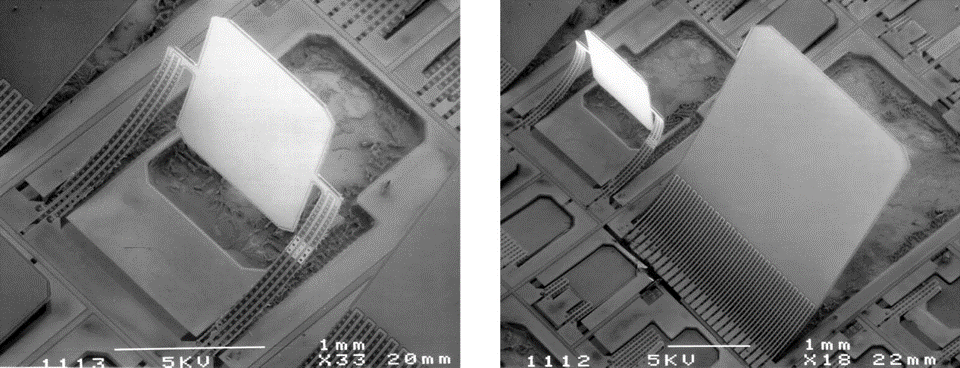
\includegraphics[width=.8\textwidth]{figures/Microspectrometer based on a tunable optical filter of porous silicon_2.png} %插入图片,[]中设置图片大小,{}中是图片文件名
        \caption{仪器结构示意图} %最终文档中希望显示的图片标题
    \end{figure}
\end{frame}

\begin{frame}[c]
    \frametitle{基于多孔硅可调谐光学滤光片的微光谱仪:原理和制造过程}
    \begin{description}
        \item[原理] 通过调节多孔硅的孔隙率可以改变其折射率,以此来制作反射镜形成法布里-珀罗滤光片。通过调节机械臂的角度改变光的入射角度,从而调节峰值波长。
    \end{description}

    工艺流程:
    \begin{itemize}
        \item $\mathrm{Si}_3\mathrm{N}_4$ 掩膜确定硅基底上多孔化和电抛光的区域
        \item 电化学刻蚀(氢氟酸和乙醇)形成多孔硅
        \item 电解抛光
        \item 在空气中晾干
        \item 充分氧化
    \end{itemize}

    \begin{columns}
        \begin{column}{.3\textwidth}
            \begin{figure}[!htb] %H为当前位置,!htb为忽略美学标准,htbp为浮动图形
                \centering %图片居中
                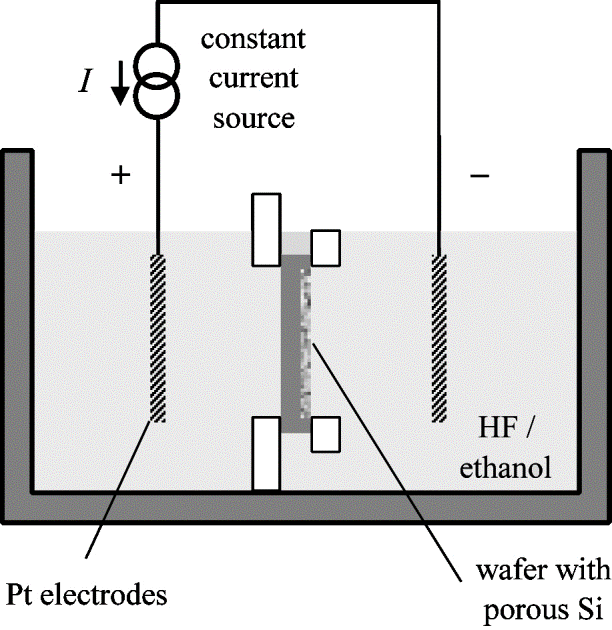
\includegraphics[width=1.\textwidth]{figures/Microspectrometer based on a tunable optical filter of porous silicon_5.png} %插入图片,[]中设置图片大小,{}中是图片文件名
                \caption{硅片多孔化和电解抛光的电化学腐蚀池} %最终文档中希望显示的图片标题
            \end{figure}
        \end{column}
        \begin{column}{.4\textwidth}
            \begin{figure}[!htb] %H为当前位置,!htb为忽略美学标准,htbp为浮动图形
                \centering %图片居中
                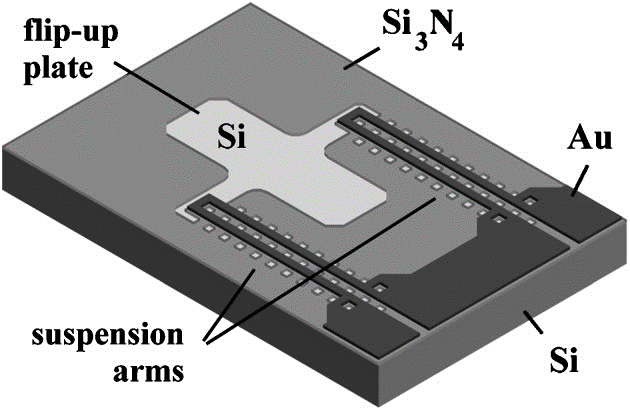
\includegraphics[width=1.\textwidth]{figures/Microspectrometer based on a tunable optical filter of porous silicon_6.png} %插入图片,[]中设置图片大小,{}中是图片文件名
                \caption{氮化硅掩膜} %最终文档中希望显示的图片标题
            \end{figure}
        \end{column}
        \begin{column}{.3\textwidth}
            \begin{figure}[!htb] %H为当前位置,!htb为忽略美学标准,htbp为浮动图形
                \centering %图片居中
                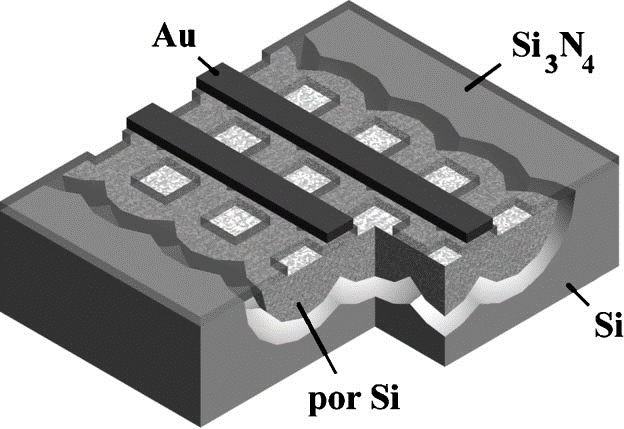
\includegraphics[width=1.\textwidth]{figures/Microspectrometer based on a tunable optical filter of porous silicon_7.png} %插入图片,[]中设置图片大小,{}中是图片文件名
                \caption{电化学刻蚀处理机械臂截面} %最终文档中希望显示的图片标题
            \end{figure}
        \end{column}
    \end{columns}
\end{frame}

\begin{frame}[c]
    \frametitle{基于多孔硅可调谐光学滤光片的微光谱仪:效果}
    \begin{figure}[!htb] %H为当前位置,!htb为忽略美学标准,htbp为浮动图形
        \centering %图片居中
        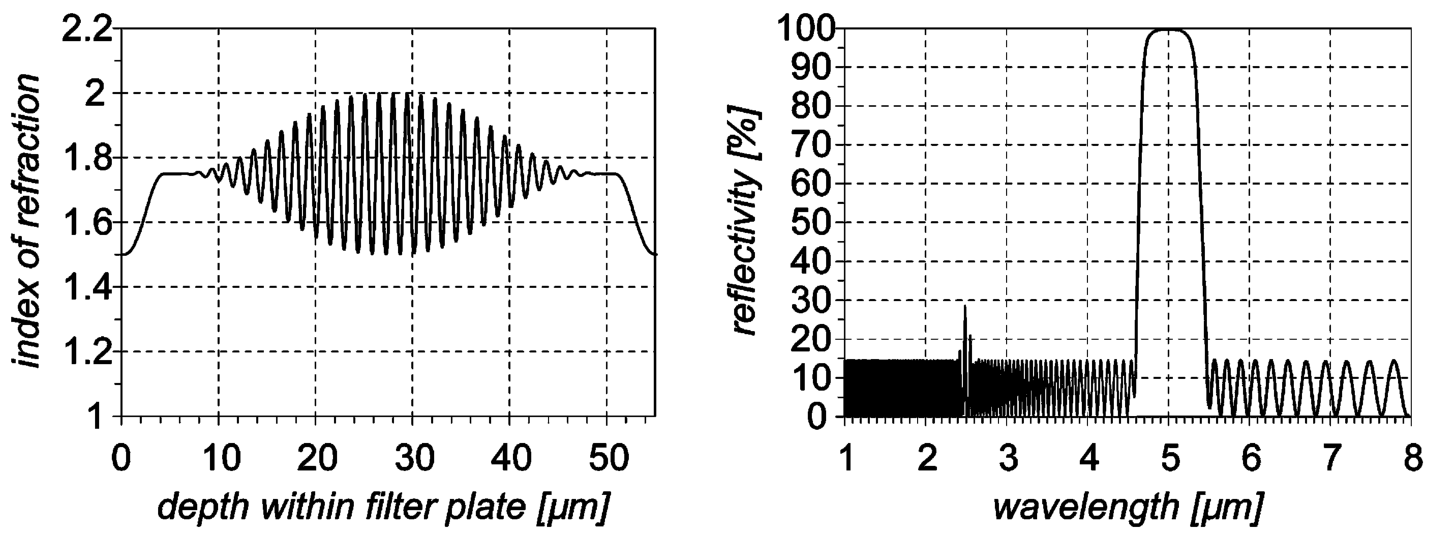
\includegraphics[width=.75\textwidth]{figures/Microspectrometer based on a tunable optical filter of porous silicon_3.png} %插入图片,[]中设置图片大小,{}中是图片文件名
        \caption{可调的折射率和反射镜的反射率} %最终文档中希望显示的图片标题
    \end{figure}
    \begin{itemize}
        \item 通过反射镜的性质可以看到工作波长在 $\lambda=5\ \mathrm{\mu m}$ 左右,范围约 $1\ \mathrm{\mu m}$。
    \end{itemize}

    \begin{columns}
        \begin{column}{.5\textwidth}
            峰值波长关系:\[\lambda_{\theta}=\lambda_0\sqrt{1-(\frac{\sin\theta}{n})^2},\ \lambda_0=2dm\]
        \end{column}
        \begin{column}{.5\textwidth}
            \begin{figure}[!htb] %H为当前位置,!htb为忽略美学标准,htbp为浮动图形
                \centering %图片居中
                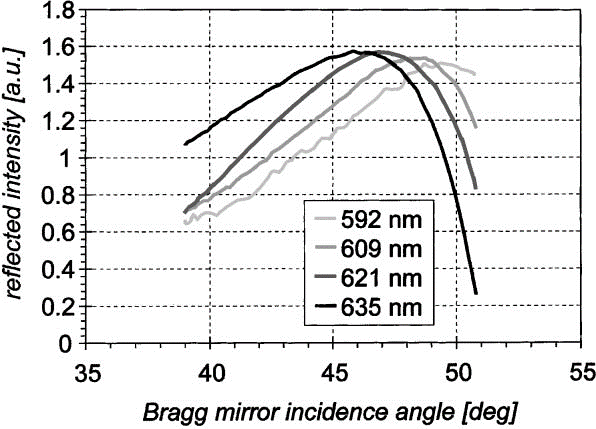
\includegraphics[width=.75\textwidth]{figures/Microspectrometer based on a tunable optical filter of porous silicon_4.png} %插入图片,[]中设置图片大小,{}中是图片文件名
                \caption{峰值波长和角度的关系} %最终文档中希望显示的图片标题
            \end{figure}
        \end{column}
    \end{columns}
\end{frame}


\subsection{窄带滤波器阵列}
\subsubsection{金属-介质单腔}
\begin{frame}[c]
    \frametitle{单片CMOS光学显微光谱仪}
    \begin{columns}
        \begin{column}{.7\textwidth}
            \begin{itemize}
                \item Correia, J.;  De Graaf, G.;  Kong, S.;  Bartek, M.; Wolffenbuttel, R., \textcolor{red}{Single-chip CMOS} optical microspectrometer. Sensors and Actuators A: Physical 2000, 82 (1-3), 191-197.
                \item \textcolor{blue}{重要性:}许多应用,例如通过光学吸收和发射线表征进行化学分析的系统,将受益于低成本单芯片光谱仪的可用性。
                \item \textcolor{blue}{创新点:}结果是芯片可以仅使用四个外部连接来操作,覆盖半高宽 18 nm 的光谱的可见光谱范围。
                \item \textcolor{blue}{意义:}气体和液体成分的识别、光吸收化学分析、发射线表征、比色法和生化分析是微型光谱仪可能有用的一些应用。
                \item \footnotesize{CMOS:互补金属氧化物半导体(Complementary Metal-Oxide-Semiconductor Transistor)}
            \end{itemize}
        \end{column}
        \begin{column}{.3\textwidth}
            \begin{figure}[H] %H为当前位置,!htb为忽略美学标准,htbp为浮动图形
                \centering %图片居中
                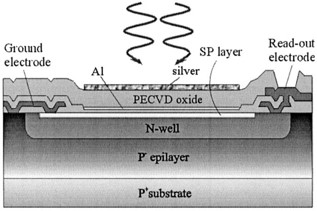
\includegraphics[width=1.\textwidth]{figures/Single-chip CMOS optical microspectrometer_1.jpg} %插入图片,[]中设置图片大小,{}中是图片文件名
            \end{figure}
            \begin{figure}[H] %H为当前位置,!htb为忽略美学标准,htbp为浮动图形
                \centering %图片居中
                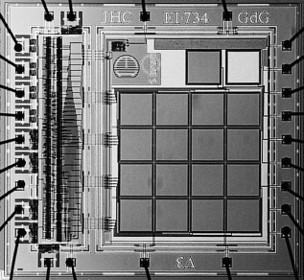
\includegraphics[width=1.\textwidth]{figures/Single-chip CMOS optical microspectrometer_2.jpg} %插入图片,[]中设置图片大小,{}中是图片文件名
            \end{figure}
        \end{column}
    \end{columns}
\end{frame}

\begin{frame}[c]
    \frametitle{单片CMOS光学显微光谱仪}
    \begin{itemize}
        \item 金属 - 介质单腔滤光片
        \item 薄膜结构:45 nm $\mathrm{Ag}$ - (225 $\sim$ 300) nm $\mathrm{SiO_2}$ - 20 nm $\mathrm{Al}$ - $\mathrm{Si}$ 基底
    \end{itemize}
    \begin{figure}[H] %H为当前位置,!htb为忽略美学标准,htbp为浮动图形
        \centering %图片居中
        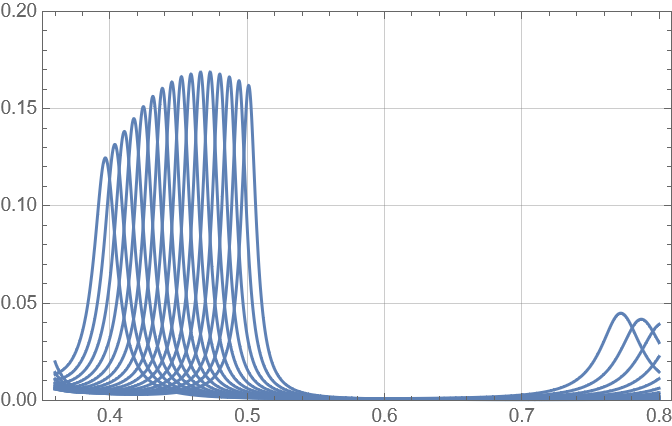
\includegraphics[width=1.\textwidth]{figures/Single-chip CMOS optical microspectrometer_3.png} %插入图片,[]中设置图片大小,{}中是图片文件名
        \caption{透射率与波长的关系} %最终文档中希望显示的图片标题
    \end{figure}
\end{frame}
\subsubsection{升级版金属-介质单腔}
\begin{frame}[c]
    \frametitle{使用集成法布里-珀罗标准具和横向针式光电探测器的 16 通道阵列型显微光谱仪}
    \begin{columns}
        \begin{column}{.5\textwidth}
            \begin{itemize}
                \item Chin-Piao, C.; Ruey-Shinq, H. In A 16-channel array-type microspectrometer using integrated \textcolor{red}{Fabry-Perot etalons} and \textcolor{purple}{lateral pin photodetectors}, SENSORS, 2003 IEEE, 22-24 Oct. 2003; 2003; pp 675-678 Vol.1.
                \item \textcolor{blue}{创新点:}工作范围几乎可以覆盖全部可见光范围。
                \item \textcolor{blue}{瓶颈:}使用空气作为谐振腔介质使得仪器需要一个桥臂做支架,因而制作更为复杂。(但是可以通过使用 $\mathrm{SiO}_2$ 代替空气来解决)
            \end{itemize}
        \end{column}
        \begin{column}{.5\textwidth}
            \begin{figure}[H] %H为当前位置,!htb为忽略美学标准,htbp为浮动图形
                \centering %图片居中
                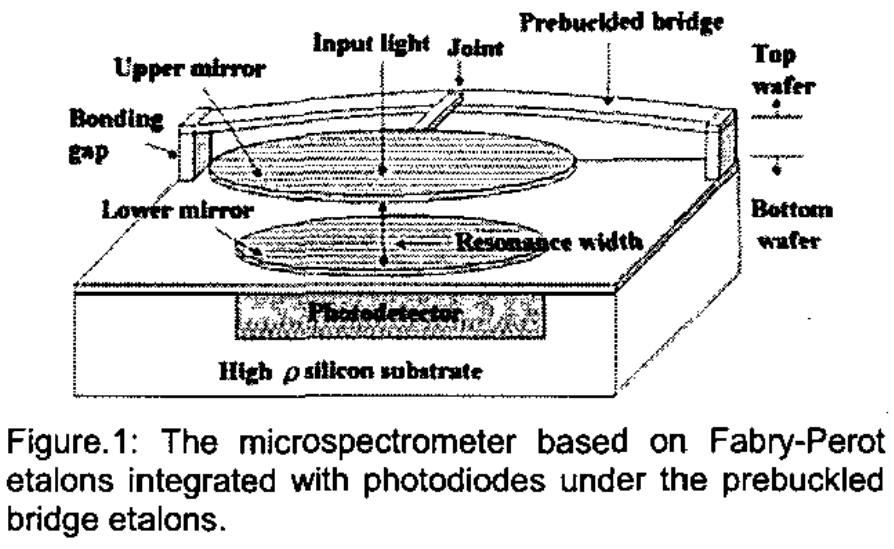
\includegraphics[width=.9\textwidth]{figures/A 16-channel array-type microspectrometer using integrated Fabry-Perot etalons and lateral pin photodetectors_1.png} %插入图片,[]中设置图片大小,{}中是图片文件名
                \caption{仪器结构示意图} %最终文档中希望显示的图片标题
            \end{figure}
            \begin{figure}[H] %H为当前位置,!htb为忽略美学标准,htbp为浮动图形
                \centering %图片居中
                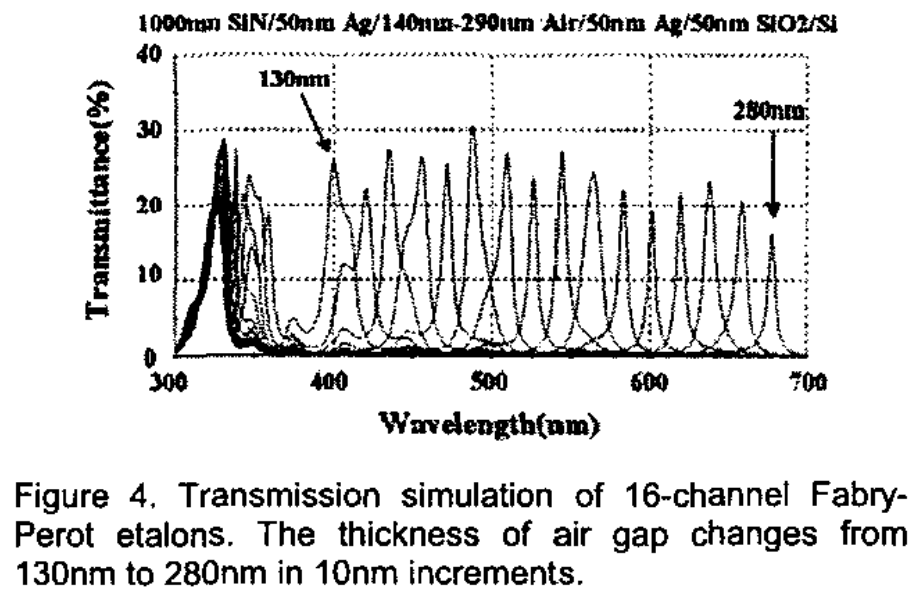
\includegraphics[width=.9\textwidth]{figures/A 16-channel array-type microspectrometer using integrated Fabry-Perot etalons and lateral pin photodetectors_2.png} %插入图片,[]中设置图片大小,{}中是图片文件名
                \caption{透射率关于波长} %最终文档中希望显示的图片标题
            \end{figure}
        \end{column}
    \end{columns}
\end{frame}

\begin{frame}[c]
    \frametitle{使用集成法布里-珀罗标准具和横向针式光电探测器的 16 通道阵列型显微光谱仪}
    \begin{itemize}
        \item 原文的膜结构:$1000 \mathrm{\ nm\ Si_3N_4} - 50 \mathrm{\ nm\ Ag} - 130\sim 280\mathrm{\ nm\ Air} - 50\mathrm{\ nm\ Ag} - 50\mathrm{\ nm\ SiO_2} - \mathrm{Si(substrate)}$
              \begin{itemize}
                  \item 其中顶层 $\mathrm{Si_3N_4}$ 是用来沉积 $\mathrm{Ag}$ 的。
                  \item 如果中间谐振腔由空气换为 $\mathrm{SiO_2}$,则无需这层 $\mathrm{Si_3N_4}$。
              \end{itemize}
        \item 改进后的膜结构:$100\mathrm{\ nm\ SiO_2} - 20 \mathrm{\ nm\ Ag} - 90\sim 200\mathrm{\ nm\ SiO_2} - 50\mathrm{\ nm\ Ag} - \mathrm{Si(substrate)}$
              \begin{itemize}
                  \item 考虑到外层的 $\mathrm{Ag}$ 容易被破坏,最外层附加 $\mathrm{100\ nm\ SiO_2}$ 作为保护。
              \end{itemize}
    \end{itemize}
    \begin{figure}[H] %H为当前位置,!htb为忽略美学标准,htbp为浮动图形
        \centering %图片居中
        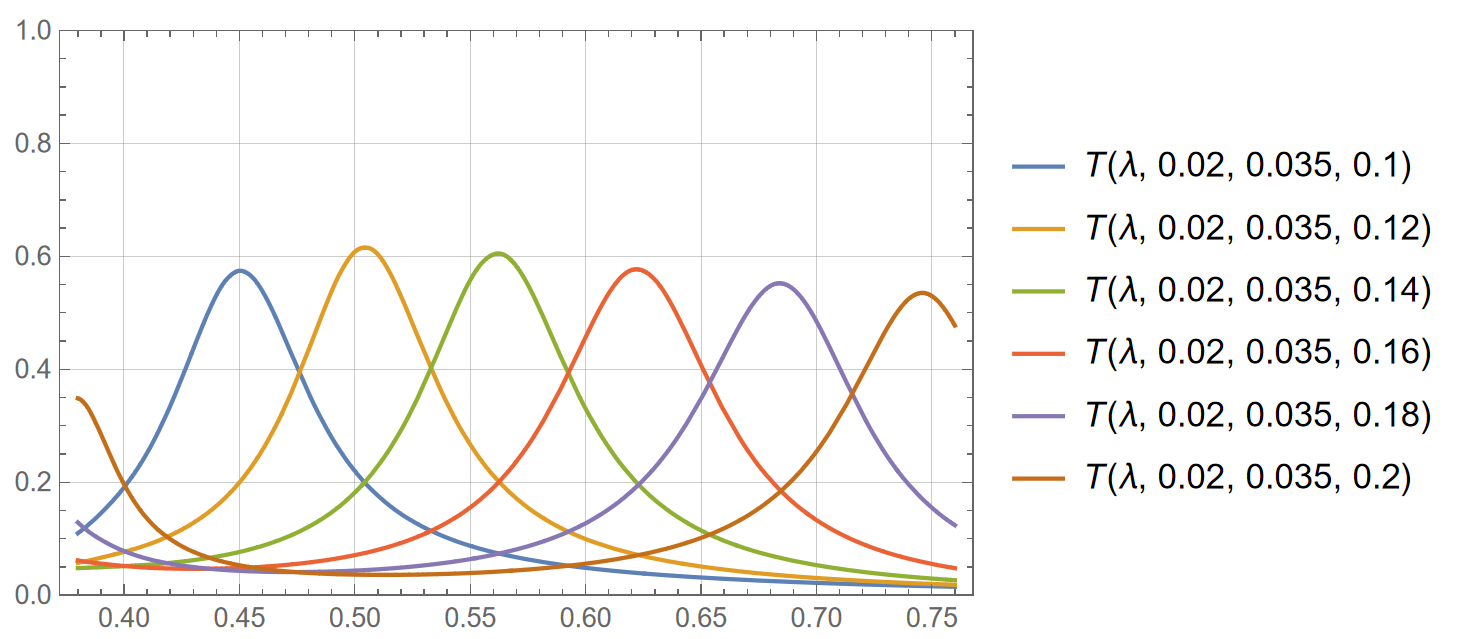
\includegraphics[width=.7\textwidth]{figures/A 16-channel array-type microspectrometer using integrated Fabry-Perot etalons and lateral pin photodetectors_3.png} %插入图片,[]中设置图片大小,{}中是图片文件名
        \caption{“改进后的膜结构”} %最终文档中希望显示的图片标题
    \end{figure}

    \begin{itemize}
        \item 若继续增加中间层 $\mathrm{SiO_2}$ 的厚度,透射峰将会出现在近红外区域,但是此时可见光短波处将会出现次级透射峰,该处的透射光将会造成较大的噪声。
    \end{itemize}
\end{frame}
\subsubsection{128 通道滤光片阵列}
\begin{frame}[c]
    \frametitle{使用集成滤光片阵列的高分辨率微型光谱仪的概念}
    \begin{columns}
        \begin{column}{.7\textwidth}
            \begin{itemize}
                \item Wang, S.-W.;  Xia, C.;  Chen, X.;  Lu, W.;  Li, M.;  Wang, H.;  Zheng, W.; Zhang, T., Concept of a \textcolor{purple}{high-resolution miniature spectrometer} using an \textcolor{red}{integrated filter array}. Optics letters 2007, 32 (6), 632-634.
                \item \textcolor{blue}{瓶颈:}滤光片阵列和 CCD 或检测器阵列之间可能会发生不对准,特别是对于具有非常小的元件尺寸和大集成度的滤光片阵列。边缘上的某些滤光片元件将与较少的 CCD 像素匹配,从而导致这些通道获得的信号较弱,并导致光谱中这些波长的信噪比相对较低。
                \item \textcolor{blue}{创新点:}同时具有极低的有效载荷、高分辨率和高可靠性等优点。
                \item 滤光片阵列具体结构(在下一篇文章中),CCD:SONY-ICX409AK
                \item \footnotesize{CCD:电荷耦合器件(Charge }Coupled Device)
            \end{itemize}
        \end{column}
        \begin{column}{.3\textwidth}
            \begin{figure}[H] %H为当前位置,!htb为忽略美学标准,htbp为浮动图形
                \centering %图片居中
                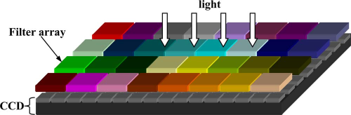
\includegraphics[width=1.\textwidth]{figures/Concept of a high-resolution miniature spectrometer using an integrated filter array_1.png} %插入图片,[]中设置图片大小,{}中是图片文件名
            \end{figure}
            \begin{figure}[H] %H为当前位置,!htb为忽略美学标准,htbp为浮动图形
                \centering %图片居中
                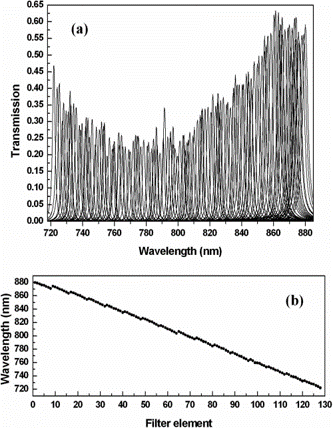
\includegraphics[width=1.\textwidth]{figures/Concept of a high-resolution miniature spectrometer using an integrated filter array_2.png} %插入图片,[]中设置图片大小,{}中是图片文件名
            \end{figure}
        \end{column}
    \end{columns}
\end{frame}

\begin{frame}[c]
    \frametitle{采用组合沉积技术快速制造128通道集成滤波器阵列}
    \begin{itemize}
        \item Wang, S.-W.;  Li, M.;  Xia, C.-S.;  Wang, H.-Q.;  Chen, X.-S.; Lu, W., \textcolor{purple}{128 channels of integrated filter array} rapidly fabricated by using the \textcolor{red}{combinatorial deposition technique}. Applied Physics B 2007, 88 (2), 281-284.
        \item \textcolor{blue}{创新点:}截至当时(2007)制作滤波器阵列最高效的组合方法。
        \item \textcolor{blue}{意义:}组合沉积技术(CDT)相对组合刻蚀技术(CET)简化了制备过程,减少了影响滤波器性能的因素。
    \end{itemize}
    \begin{figure}[H] %H为当前位置,!htb为忽略美学标准,htbp为浮动图形
        \centering %图片居中
        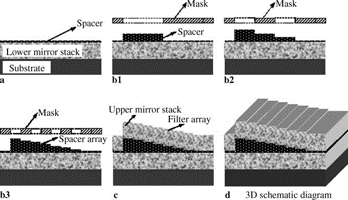
\includegraphics[width=1.\textwidth]{figures/128 channels of integrated filter array rapidly fabricated by using the combinatorial deposition technique_1.png} %插入图片,[]中设置图片大小,{}中是图片文件名
    \end{figure}
\end{frame}

\begin{frame}[c]
    \frametitle{128通道滤光片阵列}
    \begin{itemize}
        \item 全介质介质单腔滤光片
        \item 介质材料:H - $\mathrm{Nb_2O_5}$, L - $\mathrm{SiO_2}$, 中间介质 - $\mathrm{SiO_2}$
        \item 目标波长 $\lambda = 774 \text{nm}, \lambda/4 = 193.5 \text{nm}$
        \item 薄膜结构(共计29层):\begin{itemize}
                  \item 高反射膜堆 [L(193.5 nm)H(193.5 nm)LHLHLHLHLHLH]
                  \item (3.4 $\sim$ 5.1) $\times$ L(193.5 nm)
                  \item 高反射膜堆 [H(193.5 nm)L(193.5 nm)HLHLHLHLHLHL]
                  \item $\mathrm{Si}$ 基底
              \end{itemize}
    \end{itemize}
    \begin{columns}
        \begin{column}{.5\textwidth}
            \begin{figure}[H] %H为当前位置,!htb为忽略美学标准,htbp为浮动图形
                \centering %图片居中
                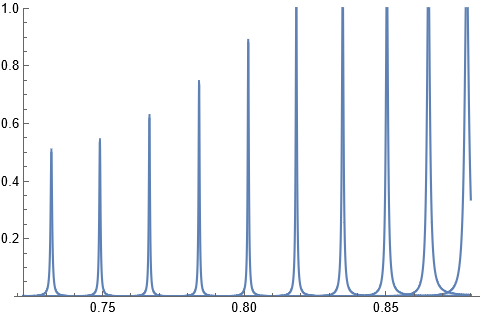
\includegraphics[width=1.\textwidth]{figures/128 channels of integrated filter array rapidly fabricated by using the combinatorial deposition technique_2.png} %插入图片,[]中设置图片大小,{}中是图片文件名
                \caption{10 通道} %最终文档中希望显示的图片标题
            \end{figure}
        \end{column}
        \begin{column}{.5\textwidth}
            \begin{figure}[H] %H为当前位置,!htb为忽略美学标准,htbp为浮动图形
                \centering %图片居中
                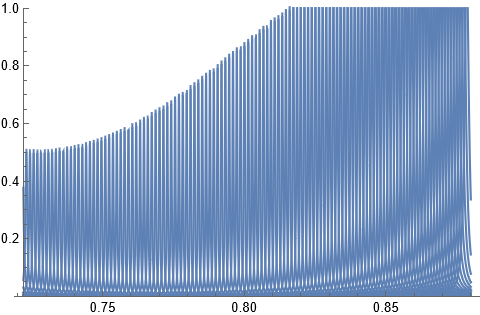
\includegraphics[width=1.\textwidth]{figures/128 channels of integrated filter array rapidly fabricated by using the combinatorial deposition technique_3.png} %插入图片,[]中设置图片大小,{}中是图片文件名
                \caption{128 通道} %最终文档中希望显示的图片标题
            \end{figure}
        \end{column}
    \end{columns}
\end{frame}

\begin{frame}[c]
    \frametitle{128通道滤光片阵列}
    \begin{itemize}
        \item 介质材料:H - $\mathrm{Nb_2O_5}$, L - $\mathrm{SiO_2}$, 中间介质 - $\mathrm{SiO_2}$
        \item 目标波长 $\lambda = 774 nm, \lambda/4 = 193.5 nm$
        \item 薄膜结构(共计29层):\\- 高反射膜堆(LHLHLHLHLHLHLH)\\- (3.4 $\sim$ 5.1) nm L\\- 高反射膜堆(HLHLHLHLHLHLHL)\\- $\mathrm{Si}$ 基底
    \end{itemize}
    \begin{figure}[H] %H为当前位置,!htb为忽略美学标准,htbp为浮动图形
        \centering %图片居中
        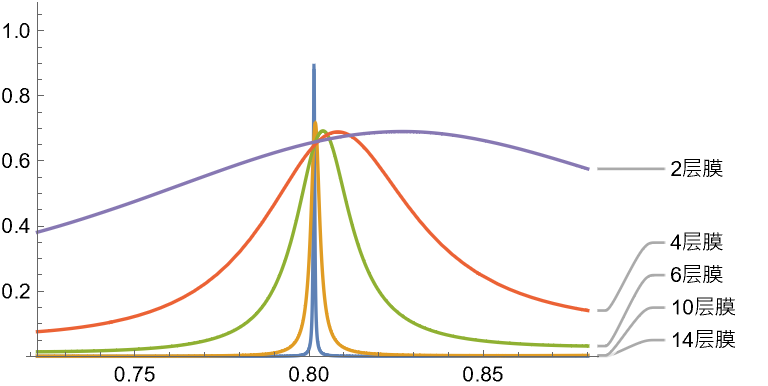
\includegraphics[width=.9\textwidth]{figures/128 channels of integrated filter array rapidly fabricated by using the combinatorial deposition technique_4.png} %插入图片,[]中设置图片大小,{}中是图片文件名
        \caption{高反射膜堆层数与透射率的关系} %最终文档中希望显示的图片标题
    \end{figure}
\end{frame}
\subsubsection{120 层蓝色滤光片}
\begin{frame}[c]
    \frametitle{用于基于白光 LED 的可见光通信系统的高性能蓝色滤光片}
    \begin{columns}
        \begin{column}{.7\textwidth}
            \begin{itemize}
                \item Wang, S.-W.;  Chen, F.;  Liang, L.;  He, S.;  Wang, Y.;  Chen, X.; Lu, W., A \textcolor{red}{high-performance blue filter} for a white-led-based \textcolor{purple}{visible light communication} system. IEEE wireless communications 2015, 22 (2), 61-67.
                \item \textcolor{blue}{重要性:}基于白光 LED 的可见光通信 (VLC) 系统提供同时照明和高速数据传输,具有高带宽、免许可、低功耗、无电磁干扰、对人体无伤害、高安全性和隐私性等诸多优点。
                \item \textcolor{blue}{创新点:}高目标透射率、尖锐精确的截止边缘、宽阻带。
                \item \textcolor{blue}{瓶颈:}面积大,等效电容高,无法应用于高速运行的情形
                \item \textcolor{blue}{意义:}有效地抑制磷光和环境光成分,提高信噪比、降低误码率,大大提高了 VLC 系统在阳光下或户外使用的能力。
                \item \footnotesize{SNR: Signal Noise Ratio(信噪比),VLC: visible light communication(可见光通信)}
                \item \footnotesize{使用 OptiLayer 软件进行薄膜设计}
            \end{itemize}
        \end{column}
        \begin{column}{.3\textwidth}
            \begin{figure}[H] %H为当前位置,!htb为忽略美学标准,htbp为浮动图形
                \centering %图片居中
                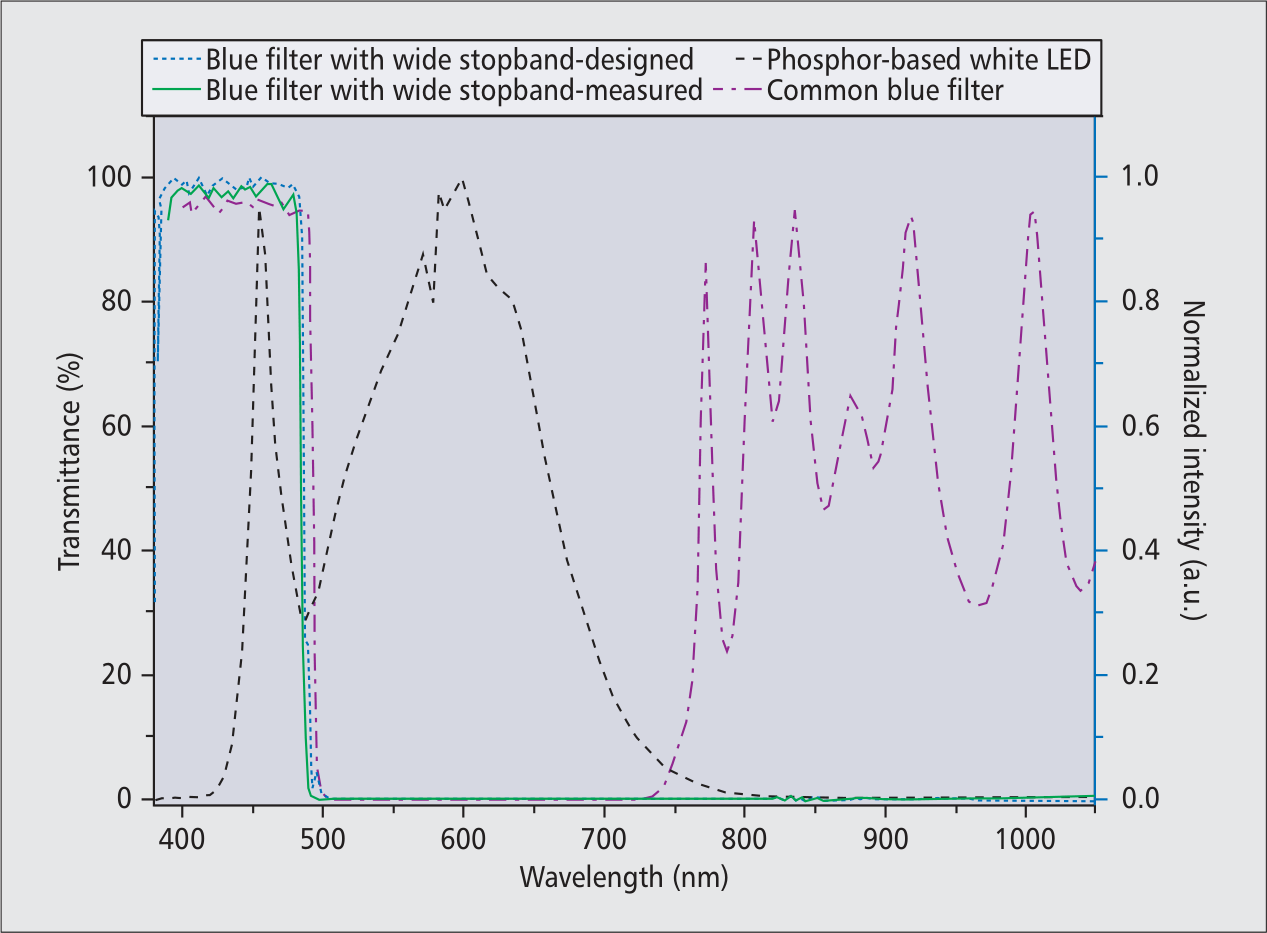
\includegraphics[width=1.1\textwidth]{figures/A high-performance blue filter for a white-led-based visible light communication system_1.png} %插入图片,[]中设置图片大小,{}中是图片文件名
                \caption{透射率} %最终文档中希望显示的图片标题
            \end{figure}
            \begin{figure}[H] %H为当前位置,!htb为忽略美学标准,htbp为浮动图形
                \centering %图片居中
                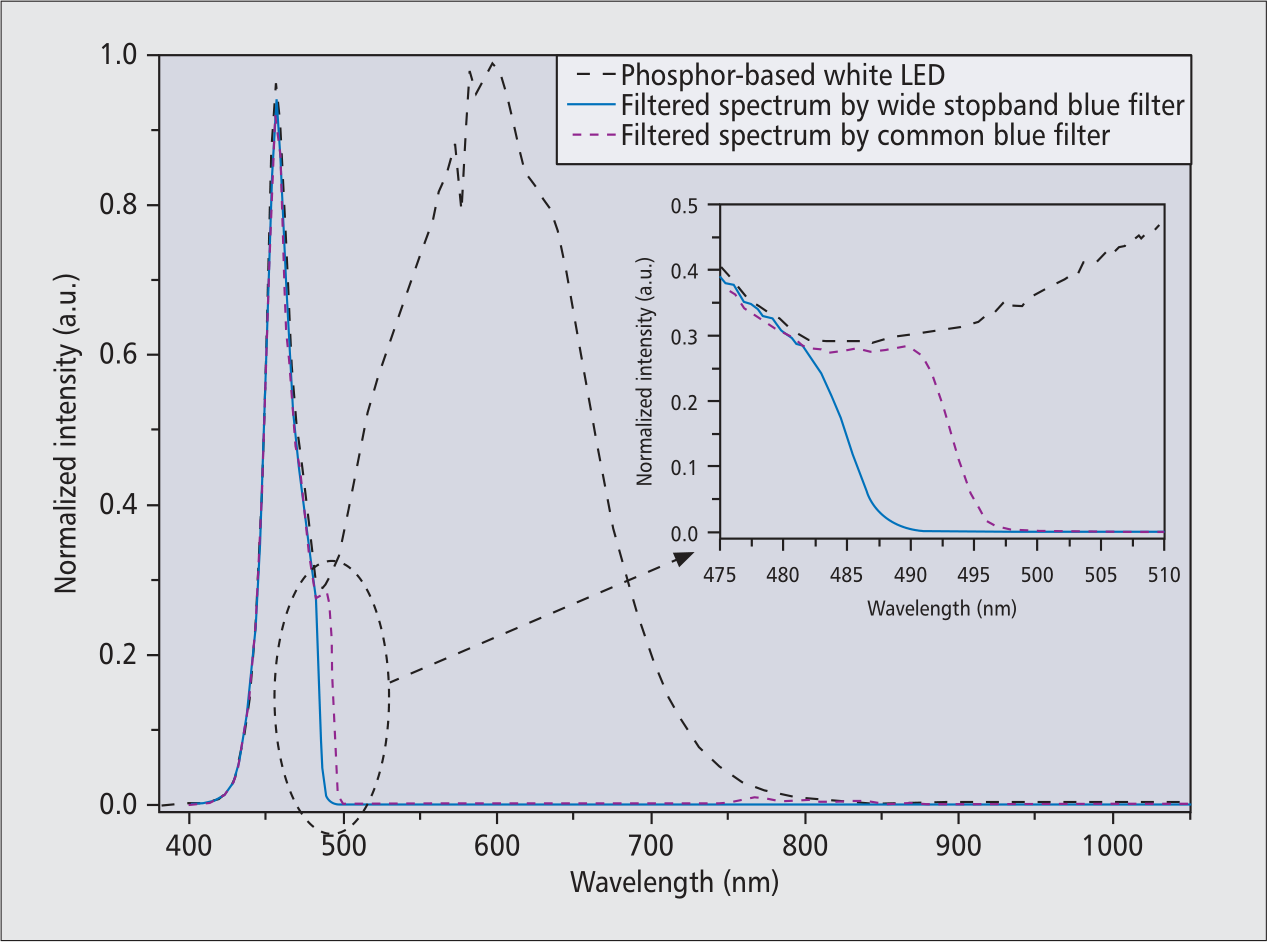
\includegraphics[width=1.1\textwidth]{figures/A high-performance blue filter for a white-led-based visible light communication system_2.png} %插入图片,[]中设置图片大小,{}中是图片文件名
                \caption{光照强度} %最终文档中希望显示的图片标题
            \end{figure}
        \end{column}
    \end{columns}
\end{frame}

\begin{frame}[c]
    \frametitle{用于基于白光 LED 的可见光通信系统的高性能蓝色滤光片}
    一点疑惑:在用文中给出的薄膜结构计算时,只有在忽略介质对光的吸收的情况下才能得到文中的结果,计及介质吸收效应时,薄膜效果极差。
    \begin{columns}
        \begin{column}{.5\textwidth}
            \begin{figure}[H] %H为当前位置,!htb为忽略美学标准,htbp为浮动图形
                \centering %图片居中
                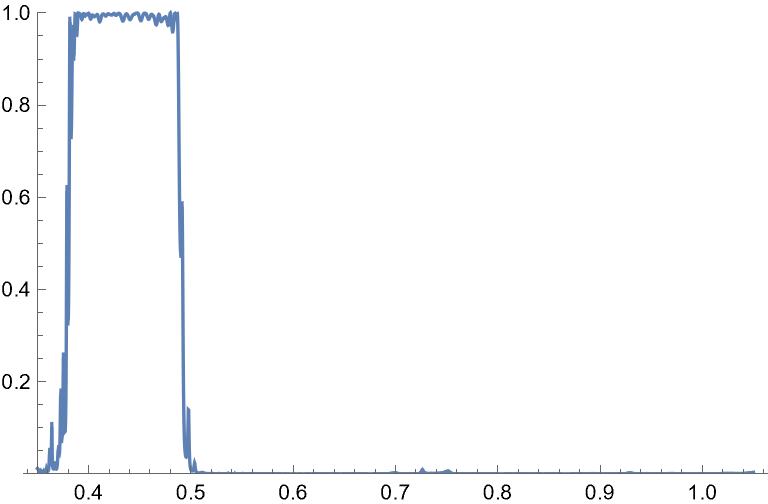
\includegraphics[width=1.\textwidth]{figures/A high-performance blue filter for a white-led-based visible light communication system_3.png} %插入图片,[]中设置图片大小,{}中是图片文件名
                \caption{不考虑介质吸收} %最终文档中希望显示的图片标题
            \end{figure}
        \end{column}
        \begin{column}{.5\textwidth}
            \begin{figure}[H] %H为当前位置,!htb为忽略美学标准,htbp为浮动图形
                \centering %图片居中
                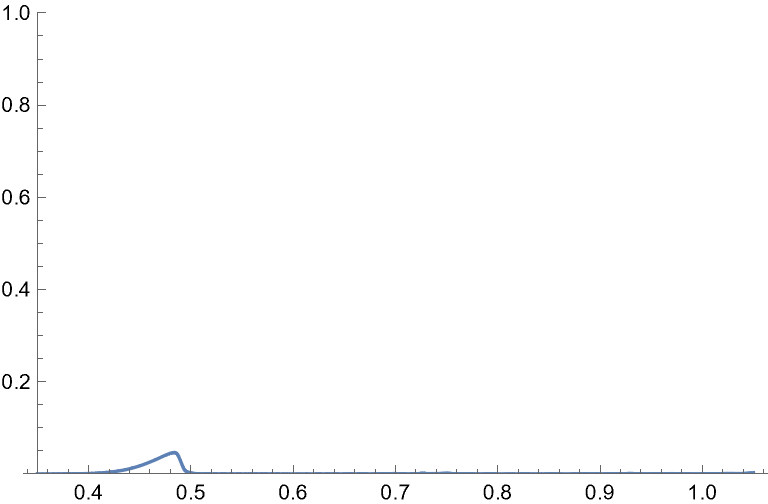
\includegraphics[width=1.\textwidth]{figures/A high-performance blue filter for a white-led-based visible light communication system_4.png} %插入图片,[]中设置图片大小,{}中是图片文件名
                \caption{考虑介质吸收} %最终文档中希望显示的图片标题
            \end{figure}
        \end{column}
    \end{columns}
\end{frame}
\subsubsection{光子晶体}
\begin{frame}[c]
    \frametitle{光子晶体光谱仪}
    \begin{columns}
        \begin{column}{.7\textwidth}
            \begin{itemize}
                \item Pervez, N. K.;  Cheng, W.;  Jia, Z.;  Cox, M. P.;  Edrees, H. M.; Kymissis, I., \textcolor{red}{Photonic crystal} spectrometer. Optics express 2010, 18 (8), 8277-8285.
                \item \textcolor{blue}{创新点:}对阵列响应的确定性控制、小尺寸、计算得到宽带光谱,成本极低。
                \item \textcolor{blue}{意义:}消费者应用,例如彩色印刷和彩色涂料匹配中的监测和反馈。
                \item \footnotesize{该作者还有一篇相似的文章待读:\url{https://doi.org/10.1364/OE.21.004411}}
                \item 使用的材料:聚甲基丙烯酸甲酯(英语:poly (methyl methacrylate),缩写:PMMA)
            \end{itemize}
        \end{column}
        \begin{column}{.3\textwidth}
            \begin{figure}[H] %H为当前位置,!htb为忽略美学标准,htbp为浮动图形
                \centering %图片居中
                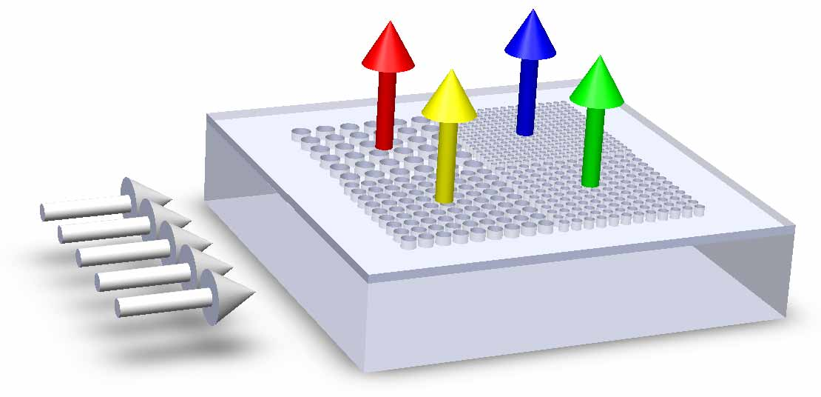
\includegraphics[width=1.\textwidth]{figures/Photonic crystal spectrometer_1.png} %插入图片,[]中设置图片大小,{}中是图片文件名
            \end{figure}
            \begin{figure}[H] %H为当前位置,!htb为忽略美学标准,htbp为浮动图形
                \centering %图片居中
                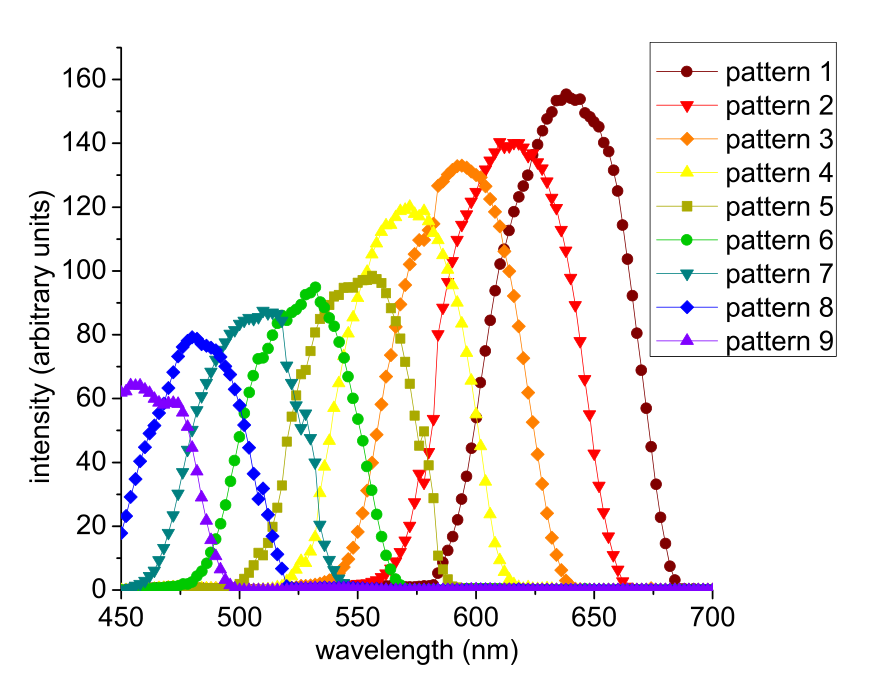
\includegraphics[width=1.\textwidth]{figures/Photonic crystal spectrometer_2.png} %插入图片,[]中设置图片大小,{}中是图片文件名
            \end{figure}
            \begin{figure}[H] %H为当前位置,!htb为忽略美学标准,htbp为浮动图形
                \centering %图片居中
                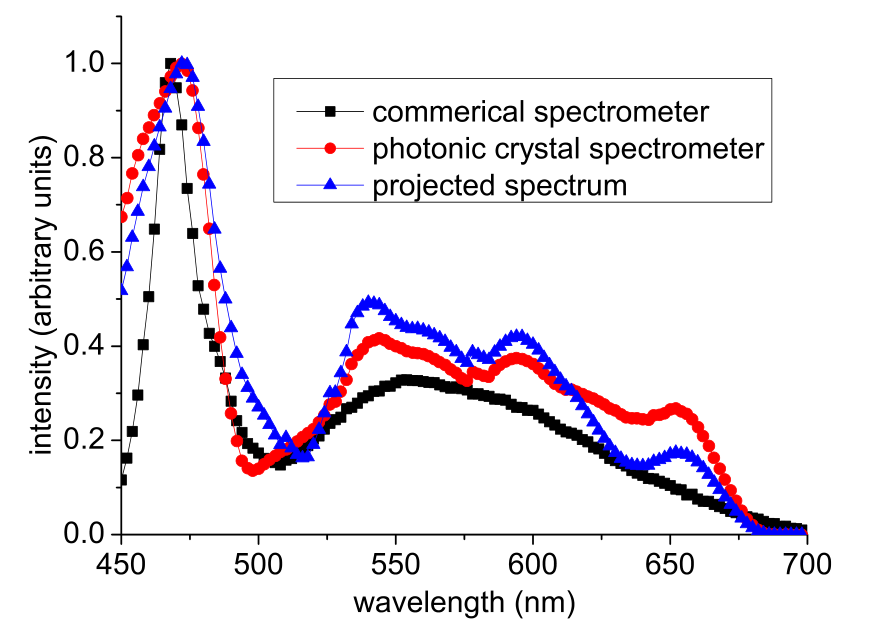
\includegraphics[width=1.\textwidth]{figures/Photonic crystal spectrometer_3.png} %插入图片,[]中设置图片大小,{}中是图片文件名
            \end{figure}
        \end{column}
    \end{columns}
\end{frame}

\begin{frame}[c]
    \frametitle{光子晶体光谱仪}
    \begin{columns}
        \begin{column}{.7\textwidth}
            \begin{itemize}
                \item Pervez, N. K.;  Cheng, W.;  Jia, Z.;  Cox, M. P.;  Edrees, H. M.; Kymissis, I., \textcolor{red}{Photonic crystal} spectrometer. Optics express 2010, 18 (8), 8277-8285.
                \item \textcolor{blue}{机理:}光子晶体由周期性电介质、金属电介质甚至超导体微结构或纳米结构组成,它们影响电磁波传播的方式与半导体晶体中的周期性电势影响电子传播的方式相同,从而确定了允许和禁止的电子能带。光子晶体包含规则重复的高折射率和低折射率区域。
                \item \textcolor{blue}{简化模型:}周期性连续变化的折射率:光子晶体 $\rightarrow$ 周期性离散变化的折射率:薄膜结构
            \end{itemize}
        \end{column}
        \begin{column}{.3\textwidth}
            \begin{figure}[H] %H为当前位置,!htb为忽略美学标准,htbp为浮动图形
                \centering %图片居中
                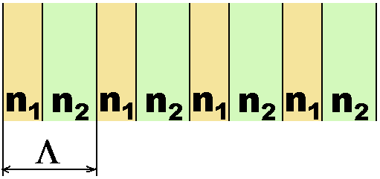
\includegraphics[width=1.\textwidth]{figures/Photonic crystal spectrometer_4.png} %插入图片,[]中设置图片大小,{}中是图片文件名
                \caption{一维光子晶体} %最终文档中希望显示的图片标题
            \end{figure}
            \begin{figure}[H] %H为当前位置,!htb为忽略美学标准,htbp为浮动图形
                \centering %图片居中
                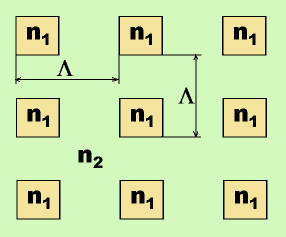
\includegraphics[width=1.\textwidth]{figures/Photonic crystal spectrometer_5.png} %插入图片,[]中设置图片大小,{}中是图片文件名
                \caption{二维光子晶体} %最终文档中希望显示的图片标题
            \end{figure}
            \begin{figure}[H] %H为当前位置,!htb为忽略美学标准,htbp为浮动图形
                \centering %图片居中
                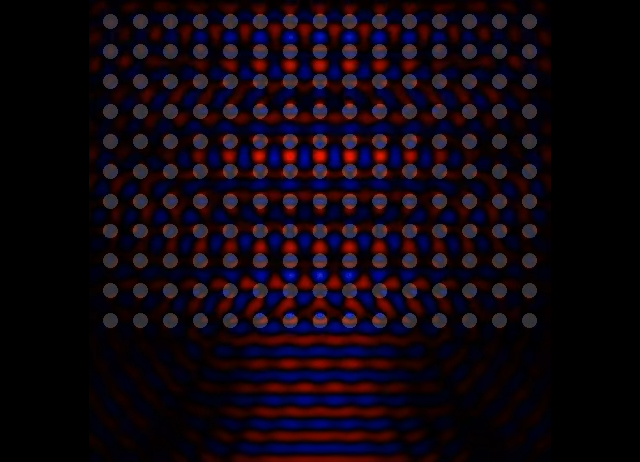
\includegraphics[width=1.\textwidth]{figures/Photonic crystal spectrometer_6.png} %插入图片,[]中设置图片大小,{}中是图片文件名
            \end{figure}
        \end{column}
    \end{columns}
\end{frame}
\subsubsection{超平面}
\begin{frame}[c]
    \frametitle{基于像素化介质超表面的分子条形码成像}
    \begin{columns}
        \begin{column}{.7\textwidth}
            \begin{itemize}
                \item Tittl, A.;  Leitis, A.;  Liu, M.;  Yesilkoy, F.;  Choi, D.-Y.;  Neshev, D. N.;  Kivshar, Y. S.; Altug, H., Imaging-based molecular barcoding with \textcolor{purple}{pixelated dielectric} \textcolor{red}{metasurfaces}. Science 2018, 360 (6393), 1105-1109.
                \item \textcolor{blue}{原理:}由吸附蛋白质前后的反射光谱变化分析蛋白质成分。
                \item \textcolor{blue}{创新点:}无需频率扫描或移动机械部件即可解析吸收指纹。
                \item \textcolor{blue}{意义:}为开发灵敏且多功能的微型中红外光谱设备铺平了道路。
                \item ?还没整明白超平面(metasurface)是什么
            \end{itemize}
        \end{column}
        \begin{column}{.3\textwidth}
            \begin{figure}[H] %H为当前位置,!htb为忽略美学标准,htbp为浮动图形
                \centering %图片居中
                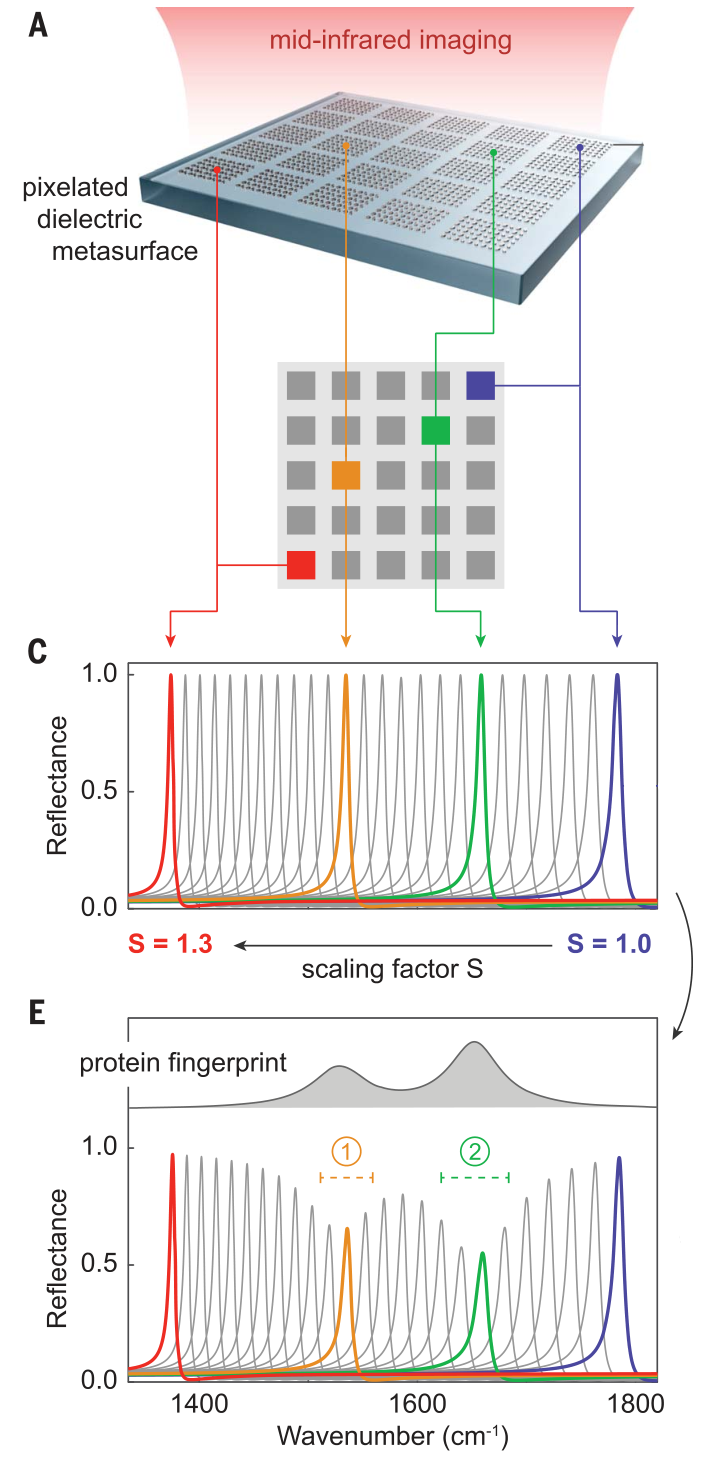
\includegraphics[width=.9\textwidth]{figures/Imaging-based molecular barcoding with pixelated dielectric metasurfaces_1.png} %插入图片,[]中设置图片大小,{}中是图片文件名
            \end{figure}
        \end{column}
    \end{columns}
    \begin{figure}[H] %H为当前位置,!htb为忽略美学标准,htbp为浮动图形
        \centering %图片居中
        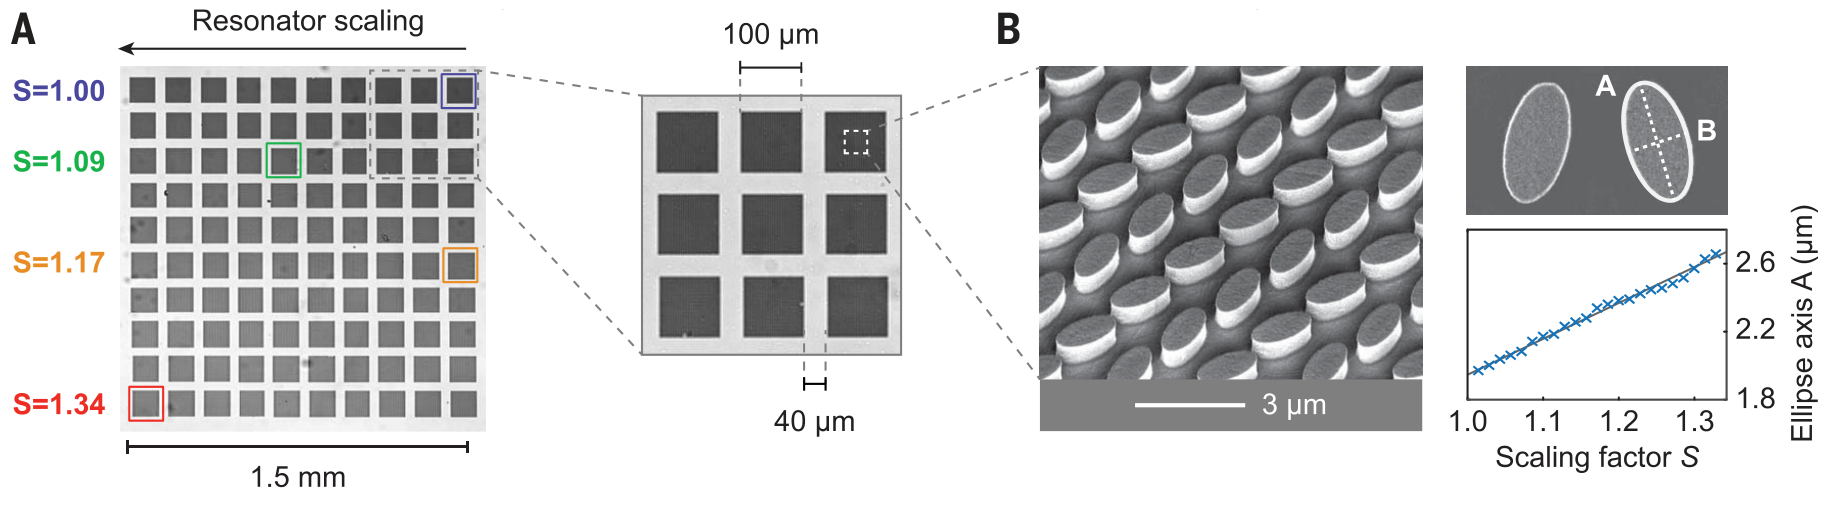
\includegraphics[width=1.\textwidth]{figures/Imaging-based molecular barcoding with pixelated dielectric metasurfaces_2.png} %插入图片,[]中设置图片大小,{}中是图片文件名
    \end{figure}
\end{frame}

\subsection{线性可变滤波器}
\subsubsection{微环谐振器}
\begin{frame}[c]
    \frametitle{使用微环谐振器的腔增强片上[测量]吸收光谱}
    \begin{itemize}
        \item Nitkowski, A.;  Chen, L.; Lipson, M., Cavity-enhanced on-chip \textcolor{purple}{absorption spectroscopy} using \textcolor{red}{microring resonators}. Optics Express 2008, 16 (16), 11930-11936.
        \item \textcolor{blue}{创新点:}使用环形谐振器,既保留了长光路,又减小了器件尺寸。
        \item \textcolor{blue}{意义:}微环谐振器可以有效地用于增加小型化片上器件的灵敏度。
        \item \textcolor{blue}{瓶颈:}仪器的信噪比仍然不够理想。
        \item \textcolor{blue}{原理:}利用环形谐振器延长光路,根据入射光谱、出射光谱和探测器接收光谱得到物质的吸收光谱。
    \end{itemize}
    \begin{columns}
        \begin{column}{.5\textwidth}
            仪器(部分)结构示意图:
            \begin{figure}[H] %H为当前位置,!htb为忽略美学标准,htbp为浮动图形
                \centering %图片居中
                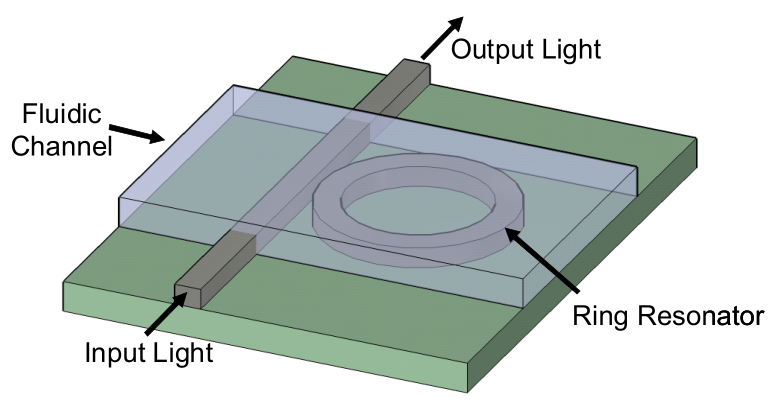
\includegraphics[width=1.\textwidth]{figures/Cavity-enhanced on-chip absorption spectroscopy using microring resonators_1.png} %插入图片,[]中设置图片大小,{}中是图片文件名
            \end{figure}
            (待测物质是液体)
        \end{column}
        \begin{column}{.5\textwidth}
            仪器原理示意图:
            \begin{figure}[H] %H为当前位置,!htb为忽略美学标准,htbp为浮动图形
                \centering %图片居中
                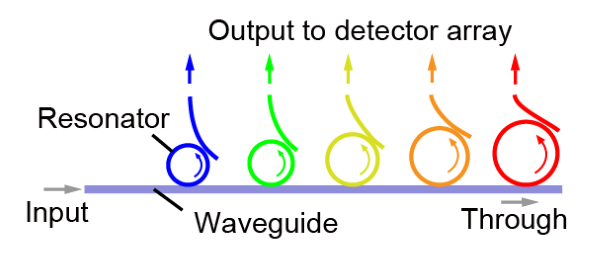
\includegraphics[width=1.\textwidth]{figures/Cavity-enhanced on-chip absorption spectroscopy using microring resonators_2.png} %插入图片,[]中设置图片大小,{}中是图片文件名
            \end{figure}
        \end{column}
    \end{columns}
\end{frame}

\begin{frame}[c]
    \frametitle{使用微环谐振器的腔增强片上[测量]吸收光谱}
    实验步骤:
    \begin{enumerate}
        \item 不注入待测物质,测量仪器固有损耗。
        \item 注入待测物质 N-methylaniline(N-甲基苯胺),测量其吸收光谱。
    \end{enumerate}
    过程细节:
    \begin{itemize}
        \item 两次实验中,入射光源分别从 1460 nm 调节到 1610 nm,步长为 1 nm。
        \item 选择该物质是因为其中的 N-H 键的吸收峰在 1500 nm 附近。
    \end{itemize}
    实验结果:
    \begin{figure}[H] %H为当前位置,!htb为忽略美学标准,htbp为浮动图形
        \centering %图片居中
        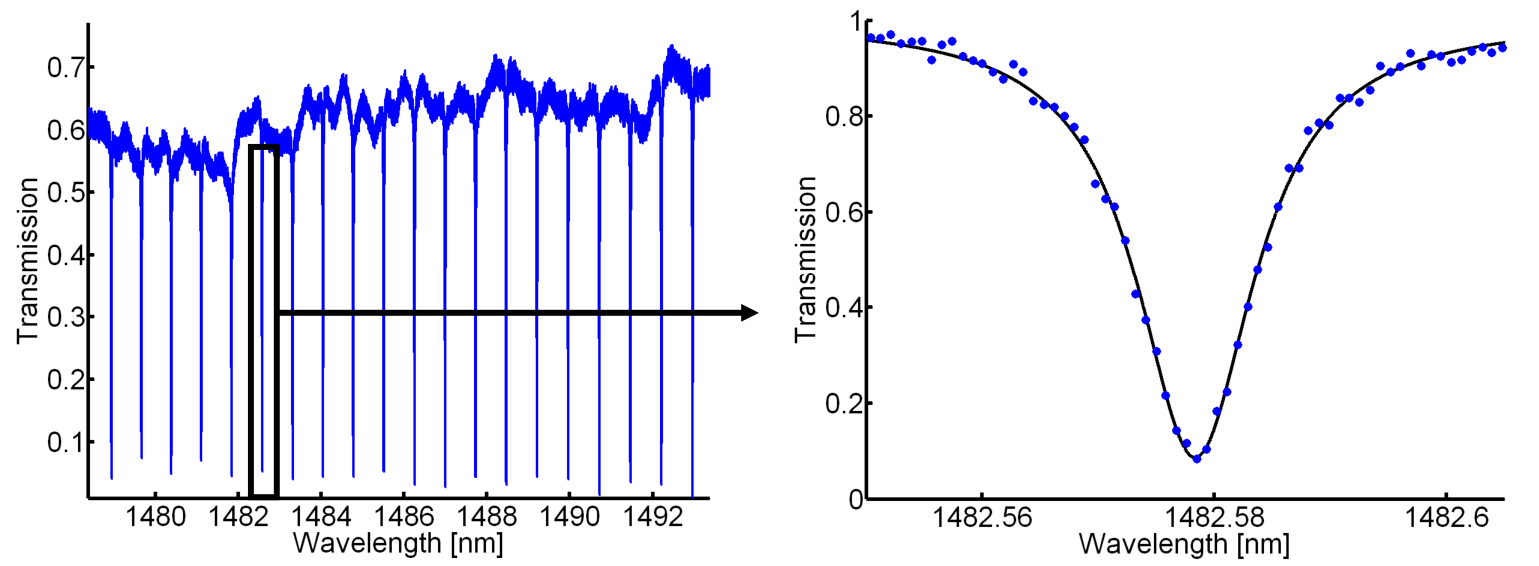
\includegraphics[width=1.\textwidth]{figures/Cavity-enhanced on-chip absorption spectroscopy using microring resonators_3.png} %插入图片,[]中设置图片大小,{}中是图片文件名
    \end{figure}
    文中还将该仪器的结果与一商用仪器相比较,两者有很好的一致性。
\end{frame}
\subsubsection{厚度梯度}
\begin{frame}[c]
    \frametitle{基于线性可变滤光片的亚纳米分辨率显微光谱仪的设计与实现}
    \begin{itemize}
        \item Emadi, A.;  Wu, H.;  de Graaf, G.; Wolffenbuttel, R., Design and implementation of a \textcolor{purple}{sub-nm resolution} microspectrometer based on a  \textcolor{red}{Linear-Variable Optical Filter}. Optics Express 2012, 20 (1), 489-507.
        \item \textcolor{blue}{创新点:}光谱分辨率基本上取决于探测器的数量。
        \item \textcolor{blue}{瓶颈:}一般用于相对狭窄的光谱波段:$610\sim 680\ \mathrm{nm}$(分辨率 0.7 nm)、$570\sim 740\ \mathrm{nm}$(分辨率 2.2 nm)。
    \end{itemize}
    仪器结构示意图:(相当于一系列连续变化的法布里-珀罗(FP)谐振腔)
    \begin{figure}[H] %H为当前位置,!htb为忽略美学标准,htbp为浮动图形
        \centering %图片居中
        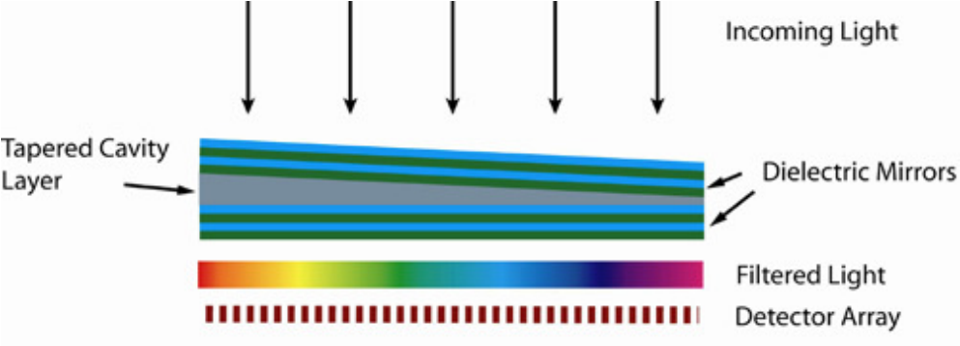
\includegraphics[width=1.\textwidth]{figures/Design and implementation of a sub-nm resolution microspectrometer based on a Linear-Variable Optical Filter_1.png} %插入图片,[]中设置图片大小,{}中是图片文件名
    \end{figure}
\end{frame}

\begin{frame}[c]
    \frametitle{基于线性可变滤光片的亚纳米分辨率显微光谱仪的设计与实现}
    薄膜结构:$\downarrow$ light
    \begin{itemize}
        \item $\mathrm{TiO}_2(68.5\ \text{nm})-\mathrm{SiO}_2(112\ \text{nm})-\mathrm{TiO}_2-\mathrm{SiO}_2-\mathrm{TiO}_2-\mathrm{SiO}_2-\mathrm{TiO}_2$
        \item $\mathrm{SiO}_2(800 \sim 1050 \text{nm})$
        \item $\mathrm{TiO}_2(68.5\ \text{nm})-\mathrm{SiO}_2(112\ \text{nm})-\mathrm{TiO}_2-\mathrm{SiO}_2-\mathrm{TiO}_2-\mathrm{SiO}_2-\mathrm{TiO}_2$
        \item Substrate: Glass
    \end{itemize}
    \begin{columns}
        \begin{column}{.5\textwidth}
            滤光效果:
            \begin{figure}[H] %H为当前位置,!htb为忽略美学标准,htbp为浮动图形
                \centering %图片居中
                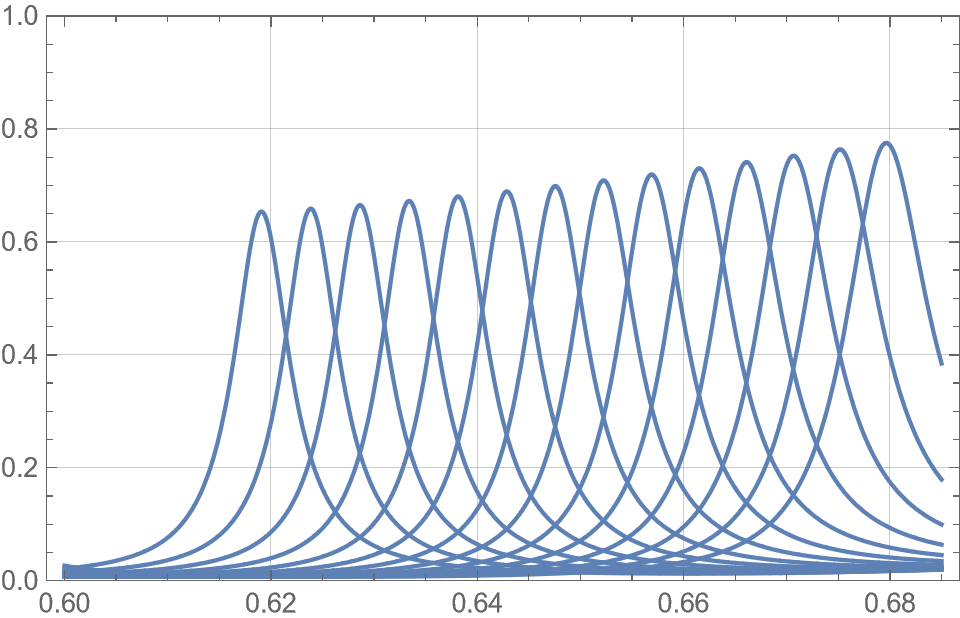
\includegraphics[width=1.\textwidth]{figures/Design and implementation of a sub-nm resolution microspectrometer based on a Linear-Variable Optical Filter_3.png} %插入图片,[]中设置图片大小,{}中是图片文件名
            \end{figure}
            沉积工艺见右(从上到下)$\rightarrow\rightarrow\rightarrow$

            文章后面还给出了数据处理的算法以及实验结果、和其他仪器的比较
        \end{column}
        \begin{column}{.5\textwidth}
            \begin{figure}[H] %H为当前位置,!htb为忽略美学标准,htbp为浮动图形
                \centering %图片居中
                \includegraphics[width=1.\textwidth]{figures/Design and implementation of a sub-nm resolution microspectrometer based on a Linear-Variable Optical Filter_2.png} %插入图片,[]中设置图片大小,{}中是图片文件名
            \end{figure}
        \end{column}
    \end{columns}
\end{frame}
\subsubsection{锥形布拉格波导}
\begin{frame}[c]
    \frametitle{基于锥形空心布拉格波导的芯片级光谱测量}
    \begin{itemize}
        \item DeCorby, R. G.;  Ponnampalam, N.;  Epp, E.;  Allen, T.; McMullin, J. N., \textcolor{purple}{Chip-scale} spectrometry based on \textcolor{red}{tapered hollow Bragg waveguides}. Optics Express 2009, 17 (19), 16632-16645
        \item \textcolor{blue}{意义:}结合了法布里-珀罗谐振腔和光栅的优势。
    \end{itemize}
    仪器结构示意图:
    \begin{figure}[H] %H为当前位置,!htb为忽略美学标准,htbp为浮动图形
        \centering %图片居中
        \includegraphics[width=1.\textwidth]{figures/Chip-scale spectrometry based on tapered hollow Bragg waveguides_1.png} %插入图片,[]中设置图片大小,{}中是图片文件名
    \end{figure}
    \begin{itemize}
        \item 原理:在某一截止位置处,特定的反射镜间距使得对应波长达到法布里珀罗谐振条件。
        \item 文章细节待读……
    \end{itemize}
\end{frame}

\section{重构技术}

\subsection{复杂的光谱到空间映射}
\subsection{色散孔阵列重构}
\begin{frame}[c]
    \frametitle{基于色散孔阵列衍射的微型光谱仪:概要}
    \begin{columns}
        \begin{column}{.6\textwidth}
            \begin{itemize}
                \item Yang, T.;  Xu, C.;  Ho, H.-p.;  Zhu, Y.-y.;  Hong, X.-h.;  Wang, Q.-j.;  Chen, Y.-c.;  Li, X.-a.;  Zhou, X.-h.;  Yi, M.-d.; Huang, W., Miniature spectrometer based on \textcolor{purple}{diffraction} in a \textcolor{red}{dispersive hole array}. Optics Letters 2015, 40 (13), 3217-3220.
                \item \textcolor{blue}{重要性:}\begin{itemize}
                          \item 不涉及运动部件、体积小、分辨率高、光谱范围宽、成本低、数据采集速度快、可靠性高;
                          \item 可以通过提高外设的计算能力来实现高分辨率、宽动态范围和实时测量能力。
                      \end{itemize}
                \item \textcolor{blue}{意义:}可以应用于生物分子识别和生物传感或通过光学吸收、荧光和发射线表征的航空航天遥测的化学分析。
                \item \textcolor{blue}{瓶颈:}\begin{itemize}
                          \item 无法集成到实验室芯片设备中;
                          \item 对于更大功率的光源需要更大的孔尺寸。
                      \end{itemize}
            \end{itemize}
        \end{column}
        \begin{column}{.4\textwidth}
            \begin{figure}[!htb] %H为当前位置,!htb为忽略美学标准,htbp为浮动图形
                \centering %图片居中
                \includegraphics[width=1.\textwidth]{figures/Miniature spectrometer based on diffraction in a dispersive hole array_1.png} %插入图片,[]中设置图片大小,{}中是图片文件名
                \caption{器件结构示意图}
            \end{figure}
        \end{column}
    \end{columns}
\end{frame}

\begin{frame}[c]
    \frametitle{基于色散孔阵列衍射的微型光谱仪:性能}
    \begin{columns}
        \begin{column}{.5\textwidth}
            建议的使用方法:
            \begin{enumerate}
                \item 在较宽的光谱范围内初步粗略测量;
                \item 再在感兴趣的波长(峰值等)附近进行精细测量。
            \end{enumerate}
            \begin{itemize}
                \item 直接在过宽的光谱范围内测量的结果不够精确;
                \item 如果直接使用更多的散射孔进行测量,虽然精度可以达到要求,但是处理数据重构光谱的时间将会增长,不利于实时应用。
            \end{itemize}
        \end{column}
        \begin{column}{.5\textwidth}
            \begin{figure}[!htb] %H为当前位置,!htb为忽略美学标准,htbp为浮动图形
                \centering %图片居中
                \includegraphics[width=1.\textwidth]{figures/Miniature spectrometer based on diffraction in a dispersive hole array_2.png} %插入图片,[]中设置图片大小,{}中是图片文件名
                \includegraphics[width=1.\textwidth]{figures/Miniature spectrometer based on diffraction in a dispersive hole array_3.png} %插入图片,[]中设置图片大小,{}中是图片文件名
                \caption{测量顺序}
            \end{figure}
        \end{column}
    \end{columns}
\end{frame}

\begin{frame}[c]
    \frametitle{基于色散孔阵列衍射的微型光谱仪:原理}
    \begin{itemize}
        \item 假设有 $n$ 个探测器(接收器),则将入射光谱按波长分为 $n$ 段,有功率关系:\[P_0=\sum^{n}_{i=1}P(\lambda_i),\ i=1,2,\dots,n\]
        \item $C_{xi}$:第 $i$ 段光谱所包含的光在第 $x$ 块探测器上的功率;
        \item $P_x=\sum^{n}_{i=1}C_{xi}P(\lambda_i),\ x=1,2,\dots,n$
        \item \[\begin{bmatrix}
                      P_1 \\P_2\\ \vdots \\ P_n
                  \end{bmatrix}=\begin{pmatrix}
                      C_{11} & C_{12} & \cdots & C_{1n} \\
                      C_{21} & C_{22} & \cdots & C_{2n} \\
                      \vdots & \vdots & \ddots & \vdots \\
                      C_{n1} & C_{n2} & \cdots & C_{nn} \\
                  \end{pmatrix}\begin{bmatrix}
                      P(\lambda_1) \\P(\lambda_2)\\ \vdots \\ P(\lambda_n)
                  \end{bmatrix}\]
        \item 理论上就是求逆矩阵,数值上涉及到稳定性等问题。
    \end{itemize}
\end{frame}

\begin{frame}[c]
    \frametitle{基于色散孔阵列衍射的微型光谱仪:类比至光学薄膜}
    \begin{itemize}
        \item 假设有 $n$ 个(带光学薄膜的)探测器(接收器),则将入射光谱按波长分为 $n$ 段,有功率关系:\[P_0=\sum^{n}_{i=1}P(\lambda_i),\ i=1,2,\dots,n\]
        \item $T_{xi}\equiv T_{x}(\lambda_i)$:第 $x$ 块光学薄膜对第 $i$ 段光谱所包含的光的透射率,亦即第 $i$ 段光谱所包含的光在第 $x$ 块(带光学薄膜的)探测器上的功率与原功率之比;
        \item $P_x=\sum^{n}_{i=1}T_{xi}P(\lambda_i),\ x=1,2,\dots,n$
        \item \[\begin{bmatrix}
                      P_1 \\P_2\\ \vdots \\ P_n
                  \end{bmatrix}=\begin{pmatrix}
                      T_{11} & T_{12} & \cdots & T_{1n} \\
                      T_{21} & T_{22} & \cdots & T_{2n} \\
                      \vdots & \vdots & \ddots & \vdots \\
                      T_{n1} & T_{n2} & \cdots & T_{nn} \\
                  \end{pmatrix}\begin{bmatrix}
                      P(\lambda_1) \\P(\lambda_2)\\ \vdots \\ P(\lambda_n)
                  \end{bmatrix}\]
        \item 对比:\begin{itemize}
                  \item 与色散孔阵列的矩阵 $C_{xi}$ 相比,光学薄膜的矩阵 $T_{xi}$ 计算更加方便,前者需要对大量的衍射结果进行求和,而后者只需根据 Fresnel 公式即可逐步计算出透射率;
                  \item 光学薄膜的设计与色散孔阵列相比更加有规律可循,并且,光学薄膜在设计好之后就已经知道它的矩阵 $T_{xi}$,但是色散孔阵列的矩阵 $C_{xi}$ 则需要在制造出之后由实验确定(理论计算可能过于复杂);
                  \item 光学薄膜的所需要的器件更多,制造更繁琐。
              \end{itemize}
    \end{itemize}
\end{frame}

\begin{frame}[c]
    \frametitle{基于色散孔阵列衍射的微型光谱仪:类比至光学薄膜}
    \begin{columns}
        \begin{column}{.4\textwidth}
            薄膜结构:\begin{itemize}
                \item $100\ \mathrm{nm\ SiO_2}$
                \item $35\ \mathrm{nm\ Ag}$
                \item $90\sim 180\ \mathrm{nm\ SiO_2}$
                \item $35\ \mathrm{nm\ Ag}$
                \item $\mathrm{Si}$
            \end{itemize}
        \end{column}
        \begin{column}{.6\textwidth}
            \begin{figure}[!htb] %H为当前位置,!htb为忽略美学标准,htbp为浮动图形
                \centering %图片居中
                \includegraphics[width=.8\textwidth]{figures/Miniature spectrometer based on diffraction in a dispersive hole array_5.pdf} %插入图片,[]中设置图片大小,{}中是图片文件名
            \end{figure}
        \end{column}
    \end{columns}
    \begin{figure}[!htb] %H为当前位置,!htb为忽略美学标准,htbp为浮动图形
        \centering %图片居中
        \includegraphics[width=1.\textwidth]{figures/Miniature spectrometer based on diffraction in a dispersive hole array_4.pdf} %插入图片,[]中设置图片大小,{}中是图片文件名
    \end{figure}
    \begin{itemize}
        \item 问题:存在这样随机生成的“探测结果”,它求解得到的“光谱分布”存在负值。
    \end{itemize}
\end{frame}


\subsection{光谱响应工程}


\section{总结}
\begin{frame}[c]
    \frametitle{理想的波长选择仪器的性质}
    \begin{columns}
        \begin{column}{.5\textwidth}
            \begin{itemize}
                \item 最小的可调时间
                \item 最小的带外传输
                \item 最小物理厚度
                \item 低功耗
                \item 对光的极化不敏感
                \item 可选择带通
                \item 完美的调制传递函数(MTF)
            \end{itemize}
        \end{column}
        \begin{column}{.5\textwidth}
            \begin{itemize}
                \item 对环境不敏感(如温度、湿度)
                \item 对入射光的入射角度不敏感(宽视场)
                \item 宽的光谱范围
                \item 透射峰高
                \item 大光圈
                \item 连续的通带
                \item 对波长的随机访问
            \end{itemize}
        \end{column}
    \end{columns}
\end{frame}

\begin{frame}[c]
    \frametitle{Application of wavelength selection}
    \begin{itemize}
        \item 光电器件
        \item (化学/生物)成分分析:\begin{itemize}
                  \item 制药工业、化学工业过程监控
                  \item 农业、生物学
                  \item 医疗诊断和保健、法医
                  \item 大气环境
              \end{itemize}
        \item 地球遥感
        \item 可见光通信
        \item 色彩视觉、艺术修复、考古
    \end{itemize}
\end{frame}

\begin{frame}[c]
    \frametitle{Acknowledgement}
    \Large{\begin{center}
            请各位老师批评指正\\
        \end{center}}
\end{frame}

\printindex
\end{document}